\documentclass[11pt, letterpaper]{article}

% Fonts and Encoding
\usepackage[utf8]{inputenc}
\usepackage[T1]{fontenc}
\usepackage{lmodern} % High-quality Latin Modern vector font

% Math and Symbols
\usepackage{amsmath, amssymb, amsthm, amsfonts, mathrsfs, mathtools}

% Layout and Geometry
\usepackage{geometry}
\geometry{letterpaper, margin=1in}
\setlength{\parindent}{0pt}
\setlength{\parskip}{0.6em}

% Formatting and Graphics
\usepackage{graphicx, xcolor, enumitem, booktabs, array, tabularx}

% TikZ for Illustrations
\usepackage{tikz}
\usetikzlibrary{arrows.meta, positioning, shapes.geometric, calc, backgrounds, matrix}

% Clickable Links and TOC
\usepackage{hyperref}
\hypersetup{
    colorlinks=true,
    linkcolor=blue,
    filecolor=magenta,      
    urlcolor=cyan,
    pdftitle={Advanced Mathematics Topic},
}

% Theorem Environments
\newtheorem{theorem}{Theorem}[section]
\newtheorem{lemma}[theorem]{Lemma}
\newtheorem{proposition}[theorem]{Proposition}
\newtheorem{corollary}[theorem]{Corollary}
\theoremstyle{definition}
\newtheorem{definition}{Definition}[section]
\newtheorem{axiom}{Axiom}[section]
\newtheorem{example}{Example}[section]
\theoremstyle{remark}
\newtheorem{remark}{Remark}[section]

% Custom Commands (Enforced standard notation)
\newcommand{\R}{\mathbb{R}}
\newcommand{\N}{\mathbb{N}}
\newcommand{\Z}{\mathbb{Z}}
\newcommand{\Q}{\mathbb{Q}}
\newcommand{\E}{\mathbb{E}}
\newcommand{\Prob}{\mathbb{P}}
\newcommand{\F}{\mathcal{F}}

\begin{document}

\title{Mastering Linear Algebra: Eigenvalues and Eigenvectors\\ \large Comprehensive Problem Sets and Detailed Solutions}
\author{Tashfeen Omran}
\date{November 16, 2026}

\maketitle
\tableofcontents
\newpage

\section{Concept Checklist and Question Mapping}

This document contains $30$ curated problems covering the complete spectrum of eigenvalue and eigenvector theory, computational mechanics, untested curriculum extensions, real-world quantitative modeling, and diagnostic error analysis. Greater weight is intentionally placed on higher-difficulty topics such as complex eigenvalues, algebraic versus geometric multiplicity, abstract matrix proofs, and applied modeling.

\begin{description}
    \item[1. Core Definition and Geometry] \hfill \\
    \textbf{Core Formula / Criterion:} $A\mathbf{x} = \lambda\mathbf{x},\ \mathbf{x} \neq \mathbf{0}$ \\
    \textbf{Key Skills and Edge Cases Tested:} Scaling along invariant spans; rejecting the zero vector $\mathbf{0}$; reversing direction ($\lambda < 0$). \\
    \textbf{Problem(s):} 1, 2, 13, 29(b)

    \item[2. Verifying an Eigenvector] \hfill \\
    \textbf{Core Formula / Criterion:} $A\mathbf{v} = \lambda\mathbf{v}$ \\
    \textbf{Key Skills and Edge Cases Tested:} Direct multiplication in $\mathbb{R}^2$ and $\mathbb{R}^3$; checking scalar consistency across components; $\lambda = 0$ case. \\
    \textbf{Problem(s):} 1, 2, 3

    \item[3. Verifying an Eigenvalue] \hfill \\
    \textbf{Core Formula / Criterion:} $(A - \lambda I)\mathbf{x} = \mathbf{0}$ \\
    \textbf{Key Skills and Edge Cases Tested:} Matrix shifting; row reducing to check for free variables; avoiding sign errors when subtracting negative diagonal entries. \\
    \textbf{Problem(s):} 4, 5

    \item[4. Eigenspace Basis Extraction] \hfill \\
    \textbf{Core Formula / Criterion:} $\operatorname{Nul}(A - \lambda I)$ \\
    \textbf{Key Skills and Edge Cases Tested:} Converting RREF to parametric vector form; fraction clearing to obtain clean integer basis vectors. \\
    \textbf{Problem(s):} 6, 7, 8, 9, 10, 12, 30(a), 30(c)

    \item[5. Multi-Dimensional Eigenspaces and Leading Free Variables] \hfill \\
    \textbf{Core Formula / Criterion:} $\dim E_\lambda \ge 1$ \\
    \textbf{Key Skills and Edge Cases Tested:} Identifying $2$D plane eigenspaces; recognizing when $x_1$ has no pivot and is a free variable. \\
    \textbf{Problem(s):} 8, 9, 17, 30(a)

    \item[6. Characteristic Equation and Full Spectrum] \hfill \\
    \textbf{Core Formula / Criterion:} $\det(A - \lambda I) = 0$ \\
    \textbf{Key Skills and Edge Cases Tested:} Computing characteristic polynomials for $2\times 2$ and $3\times 3$ matrices; finding all eigenvalues and bases. \\
    \textbf{Problem(s):} 12, 13, 14, 15, 16, 24, 25, 26, 28, 29(a)

    \item[7. Triangular Matrix Shortcut] \hfill \\
    \textbf{Core Formula / Criterion:} $\det(A - \lambda I) = \prod (a_{ii} - \lambda)$ \\
    \textbf{Key Skills and Edge Cases Tested:} Reading eigenvalues directly from main diagonals of upper/lower triangular matrices without row reducing $A$. \\
    \textbf{Problem(s):} 10, 17, 22

    \item[8. Zero Eigenvalue and Invertibility] \hfill \\
    \textbf{Core Formula / Criterion:} $\lambda = 0 \iff \det(A) = 0$ \\
    \textbf{Key Skills and Edge Cases Tested:} Connecting $\lambda = 0$ to singular matrices, dependent columns, and nontrivial null spaces. \\
    \textbf{Problem(s):} 3, 10, 11, 20, 30(b)

    \item[9. Complex Eigenvalues and Rotations] \hfill \\
    \textbf{Core Formula / Criterion:} $\lambda = \alpha \pm \beta i \in \mathbb{C}$ \\
    \textbf{Key Skills and Edge Cases Tested:} Solving $\det(A - \lambda I) = 0$ over $\mathbb{C}$; interpreting absence of real eigenvectors for rotation matrices $R_\theta$. \\
    \textbf{Problem(s):} 13, 14, 15

    \item[10. Algebraic vs.\ Geometric Multiplicity] \hfill \\
    \textbf{Core Formula / Criterion:} $\operatorname{GM}(\lambda) \le \operatorname{AM}(\lambda)$ \\
    \textbf{Key Skills and Edge Cases Tested:} Comparing root multiplicity to eigenspace dimension; classifying defective matrices; parameter tuning. \\
    \textbf{Problem(s):} 10, 16, 17, 18

    \item[11. Theoretical Proofs and Matrix Algebra] \hfill \\
    \textbf{Core Formula / Criterion:} $p(A)\mathbf{x} = p(\lambda)\mathbf{x}$ \\
    \textbf{Key Skills and Edge Cases Tested:} Independence of distinct-eigenvalue vectors; $A^{-1}$, $A+cI$, $A^k$, $A^T$, idempotent, nilpotent, and eigenbasis powers. \\
    \textbf{Problem(s):} 19, 20, 21, 22, 23, 24

    \item[12. Real-World Modeling (ML, Quant, Markov, ODEs)] \hfill \\
    \textbf{Core Formula / Criterion:} $\Sigma\mathbf{w} = \lambda\mathbf{w},\ P\boldsymbol{\pi} = \boldsymbol{\pi}$ \\
    \textbf{Key Skills and Edge Cases Tested:} PCA variance maximization via Lagrange multipliers; portfolio risk factors; PageRank steady state; ODE stability. \\
    \textbf{Problem(s):} 25, 26, 27, 28

    \item[13. Diagnostic Testing (``Find the Flaw'')] \hfill \\
    \textbf{Core Formula / Criterion:} Row ops alter $\lambda$ \\
    \textbf{Key Skills and Edge Cases Tested:} Catching row reduction of $A$, zero-vector traps, missed free variables, $\lambda = 0$ myths, and sign errors. \\
    \textbf{Problem(s):} 4, 9, 29, 30
\end{description}

\newpage

\section{Problem Sets}

\subsection{Core Definitions and Verification (Problems 1--5)}

\textbf{Problem 1 (Geometric Interpretation, Core Definition, and the Zero Vector Trap).}
Let
\[
A = \begin{bmatrix} 2 & 1 \\ 1 & 2 \end{bmatrix}, \quad \mathbf{u} = \begin{bmatrix} 1 \\ 1 \end{bmatrix}, \quad \mathbf{v} = \begin{bmatrix} 1 \\ -1 \end{bmatrix}, \quad \mathbf{w} = \begin{bmatrix} 2 \\ 0 \end{bmatrix}, \quad \mathbf{z} = \begin{bmatrix} 0 \\ 0 \end{bmatrix}.
\]
\begin{enumerate}[label=(\alph*)]
    \item Determine which of the vectors $\mathbf{u}$, $\mathbf{v}$, $\mathbf{w}$, and $\mathbf{z}$ are eigenvectors of $A$, and state the corresponding eigenvalue for each eigenvector.
    \item Explain geometrically how the linear transformation $\mathbf{x} \mapsto A\mathbf{x}$ acts on $\mathbf{u}$, $\mathbf{v}$, and $\mathbf{w}$ relative to their respective spans in $\mathbb{R}^2$.
\end{enumerate}

\textbf{Problem 2 (Verifying an Eigenvector with Direction Reversal).}
Determine whether $\mathbf{v} = \begin{bmatrix} 3 \\ -2 \end{bmatrix}$ is an eigenvector of $A = \begin{bmatrix} -1 & 3 \\ 2 & 0 \end{bmatrix}$. If it is, find the corresponding eigenvalue and describe the geometric effect of $A$ on $\mathbf{v}$.

\textbf{Problem 3 (Verifying Eigenvectors in $\mathbb{R}^3$ Including $\lambda = 0$).}
Consider the matrix and vectors
\[
A = \begin{bmatrix} 2 & -1 & 3 \\ 4 & -2 & 6 \\ -2 & 1 & 1 \end{bmatrix}, \quad \mathbf{v}_1 = \begin{bmatrix} 1 \\ 2 \\ 0 \end{bmatrix}, \quad \mathbf{v}_2 = \begin{bmatrix} 1 \\ 2 \\ 1 \end{bmatrix}.
\]
Determine whether $\mathbf{v}_1$ and $\mathbf{v}_2$ are eigenvectors of $A$. For each vector that is an eigenvector, determine its corresponding eigenvalue.

\textbf{Problem 4 (Verifying an Eigenvalue with Negative Diagonal Entries).}
Is $\lambda = -3$ an eigenvalue of $A = \begin{bmatrix} -5 & 4 \\ -1 & -1 \end{bmatrix}$? Justify your answer rigorously using $(A - \lambda I)\mathbf{x} = \mathbf{0}$, and if yes, find one corresponding eigenvector.

\textbf{Problem 5 (Verifying Eigenvalues in $\mathbb{R}^3$).}
Determine whether $\lambda = 2$ and $\lambda = 5$ are eigenvalues of
\[
A = \begin{bmatrix} 4 & -1 & 2 \\ 1 & 2 & 1 \\ -2 & 2 & 0 \end{bmatrix}.
\]
For any value that is an eigenvalue, compute one corresponding eigenvector.

\subsection{Eigenspace Extraction, Triangular Shortcuts, and Zero Eigenvalues (Problems 6--12)}

\textbf{Problem 6 (Finding Bases for $2\times 2$ Eigenspaces).}
Find a basis for each eigenspace of $A = \begin{bmatrix} 5 & -2 \\ -4 & 7 \end{bmatrix}$ corresponding to the eigenvalues $\lambda = 3$ and $\lambda = 9$.

\textbf{Problem 7 (Finding Bases for Multiple $3\times 3$ Eigenspaces with Fraction Clearing).}
Find a basis for the eigenspaces of
\[
A = \begin{bmatrix} -1 & 6 & 0 \\ 3 & 5 & -3 \\ -3 & 6 & 2 \end{bmatrix}
\]
corresponding to the eigenvalues $\lambda = -1, 2, 5$. Express each basis vector with integer entries by clearing fractions where appropriate.

\textbf{Problem 8 (Extracting a Two-Dimensional Eigenspace).}
Find a basis for each eigenspace of
\[
B = \begin{bmatrix} 6 & -2 & 2 \\ -2 & 3 & -1 \\ 2 & -1 & 3 \end{bmatrix}
\]
corresponding to $\lambda = 2$ and $\lambda = 8$, and state the geometric dimension of each eigenspace in $\mathbb{R}^3$.

\textbf{Problem 9 (Eigenspace Extraction with a Leading Free Variable).}
Find a basis for the eigenspace of
\[
A = \begin{bmatrix} 4 & -3 & 2 \\ 0 & 5 & -1 \\ 0 & 0 & 4 \end{bmatrix}
\]
corresponding to $\lambda = 4$, carefully tracking all pivot columns and free variables in the Reduced Row Echelon Form (RREF).

\textbf{Problem 10 (Triangular Matrix Shortcut and Eigenspace Extraction).}
Consider the $4 \times 4$ matrix
\[
A = \begin{bmatrix} -2 & 0 & 0 & 0 \\ 7 & 5 & 0 & 0 \\ -3 & 4 & 5 & 0 \\ 9 & -1 & 6 & 0 \end{bmatrix}.
\]
\begin{enumerate}[label=(\alph*)]
    \item Without computing cofactor expansions or row-reducing $A$, state all eigenvalues of $A$ and justify your answer.
    \item Determine whether $A$ is invertible based solely on your answer to part (a).
    \item Find a basis for the eigenspace corresponding to $\lambda = 5$.
\end{enumerate}

\textbf{Problem 11 (Zero Eigenvalue and Invertibility Criterion).}
Let $k \in \mathbb{R}$ and consider the matrix
\[
A = \begin{bmatrix} 1 & 2 & -1 \\ 3 & 5 & -1 \\ 2 & k & 4 \end{bmatrix}.
\]
\begin{enumerate}[label=(\alph*)]
    \item Find the exact value of $k$ for which $\lambda = 0$ is an eigenvalue of $A$.
    \item For that value of $k$, find a basis for the eigenspace corresponding to $\lambda = 0$ and explain how this result relates to the invertibility of $A$.
\end{enumerate}

\textbf{Problem 12 (Characteristic Equation and Full Spectrum Extraction).}
Using the characteristic equation $\det(A - \lambda I) = 0$, find all eigenvalues and a basis for each corresponding eigenspace of
\[
A = \begin{bmatrix} 2 & 1 & 1 \\ 0 & 4 & 0 \\ 3 & -1 & 0 \end{bmatrix}.
\]

\subsection{Complex Eigenvalues and Multiplicity Analysis (Problems 13--18)}

\textbf{Problem 13 (Complex Eigenvalues of a Rotation-Scaling Matrix).}
Consider the matrix $A = \begin{bmatrix} 3 & -4 \\ 4 & 3 \end{bmatrix}$.
\begin{enumerate}[label=(\alph*)]
    \item Find all eigenvalues of $A$ over $\mathbb{C}$.
    \item Explain geometrically why $A$ possesses no real eigenvectors in $\mathbb{R}^2$.
    \item Find a basis over $\mathbb{C}$ for the eigenspace corresponding to the eigenvalue with positive imaginary part.
\end{enumerate}

\textbf{Problem 14 (General Rotation Matrix in $\mathbb{R}^2$).}
Let $R_\theta = \begin{bmatrix} \cos\theta & -\sin\theta \\ \sin\theta & \cos\theta \end{bmatrix}$ represent a counterclockwise rotation in $\mathbb{R}^2$ by an angle $\theta \in (0, \pi)$.
\begin{enumerate}[label=(\alph*)]
    \item Compute the characteristic polynomial of $R_\theta$ and prove algebraically that $R_\theta$ has no real eigenvalues for $\theta \in (0, \pi)$.
    \item Find the complex eigenvalues of $R_\theta$ in both trigonometric and polar exponential form ($e^{\pm i\theta}$), and determine a complex eigenvector for each eigenvalue.
\end{enumerate}

\textbf{Problem 15 (Mixed Real and Complex Spectrum in $\mathbb{R}^3$).}
Consider the $3 \times 3$ matrix
\[
A = \begin{bmatrix} 2 & 0 & 0 \\ 1 & 1 & -2 \\ 0 & 2 & 1 \end{bmatrix}.
\]
Find all real and complex eigenvalues of $A$, and find a basis for the real eigenspace corresponding to the real eigenvalue.

\textbf{Problem 16 (Algebraic vs.\ Geometric Multiplicity and Defective Matrices).}
Let
\[
A = \begin{bmatrix} 3 & 1 & 0 \\ 0 & 3 & 0 \\ 4 & -2 & 1 \end{bmatrix}.
\]
\begin{enumerate}[label=(\alph*)]
    \item Compute the characteristic polynomial of $A$ and state the algebraic multiplicity of each eigenvalue.
    \item Find a basis for each eigenspace and state the geometric multiplicity of each eigenvalue.
    \item Determine whether $A$ is defective, and explain what this implies about the existence of an eigenvector basis for $\mathbb{R}^3$.
\end{enumerate}

\textbf{Problem 17 (Parameter Tuning for Multiplicity and Diagonalizability).}
Consider the upper-triangular matrix
\[
A = \begin{bmatrix} 2 & 1 & a \\ 0 & 5 & 3 \\ 0 & 0 & 2 \end{bmatrix},
\]
where $a \in \mathbb{R}$ is a real parameter.
\begin{enumerate}[label=(\alph*)]
    \item State the eigenvalues of $A$ and their algebraic multiplicities.
    \item Determine all values of $a$ for which the geometric multiplicity of $\lambda = 2$ equals its algebraic multiplicity (making $A$ non-defective), and all values of $a$ for which $A$ is defective.
    \item Find a basis for the eigenspace $E_2$ in both regimes.
\end{enumerate}

\textbf{Problem 18 (Inverse Construction from Prescribed Eigenvectors).}
Suppose a $2 \times 2$ matrix $A$ has eigenvectors $\mathbf{v}_1 = \begin{bmatrix} 2 \\ 1 \end{bmatrix}$ with eigenvalue $\lambda_1 = 5$, and $\mathbf{v}_2 = \begin{bmatrix} 1 \\ -1 \end{bmatrix}$ with eigenvalue $\lambda_2 = -1$.
\begin{enumerate}[label=(\alph*)]
    \item Determine the explicit matrix $A$ using $A\mathbf{v}_1 = 5\mathbf{v}_1$ and $A\mathbf{v}_2 = -\mathbf{v}_2$ (or $A = P D P^{-1}$).
    \item Decompose $\mathbf{x} = \begin{bmatrix} 5 \\ 1 \end{bmatrix}$ as a linear combination of $\mathbf{v}_1$ and $\mathbf{v}_2$ to compute $A\mathbf{x}$, and verify your answer by direct matrix multiplication.
\end{enumerate}

\subsection{Theoretical Proofs and Abstract Matrix Properties (Problems 19--24)}

\textbf{Problem 19 (Linear Independence of Eigenvectors and Bound on Distinct Eigenvalues).}
\begin{enumerate}[label=(\alph*)]
    \item Prove that if $\mathbf{v}_1$ and $\mathbf{v}_2$ are eigenvectors of an $n \times n$ matrix $A$ corresponding to distinct eigenvalues $\lambda_1 \neq \lambda_2$, then $\{\mathbf{v}_1, \mathbf{v}_2\}$ is linearly independent.
    \item Given that any set of eigenvectors corresponding to pairwise distinct eigenvalues is linearly independent, explain why an $n \times n$ matrix can have at most $n$ distinct eigenvalues.
\end{enumerate}

\textbf{Problem 20 (Eigenvalues of Inverses and Shifted Matrices).}
Let $A$ be an invertible $n \times n$ matrix, let $c \in \mathbb{R}$, and let $\lambda$ be an eigenvalue of $A$ with corresponding eigenvector $\mathbf{x}$.
\begin{enumerate}[label=(\alph*)]
    \item Prove that $\lambda \neq 0$, and show that $\lambda^{-1}$ is an eigenvalue of $A^{-1}$ with eigenvector $\mathbf{x}$, explicitly maintaining proper left-multiplication order.
    \item Prove that $\lambda + c$ is an eigenvalue of $A + cI$ with eigenvector $\mathbf{x}$.
    \item Suppose $A$ is a $3 \times 3$ matrix with eigenvalues $1$, $3$, and $-4$. Determine the eigenvalues of $(A + 2I)^{-1}$.
\end{enumerate}

\textbf{Problem 21 (Matrix Powers and Matrix Polynomials).}
Let $A$ be an $n \times n$ matrix and let $\mathbf{x} \neq \mathbf{0}$ be an eigenvector of $A$ with eigenvalue $\lambda$.
\begin{enumerate}[label=(\alph*)]
    \item Prove by mathematical induction that $A^k \mathbf{x} = \lambda^k \mathbf{x}$ for every integer $k \ge 1$.
    \item Prove that for any polynomial $p(t) = \sum_{j=0}^{m} c_j t^j$, the vector $\mathbf{x}$ is an eigenvector of the matrix $p(A) = \sum_{j=0}^{m} c_j A^j$ with eigenvalue $p(\lambda)$ (where $A^0 = I$).
    \item Suppose $\mathbf{v} = \begin{bmatrix} 1 \\ -2 \\ 1 \end{bmatrix}$ is an eigenvector of a matrix $B$ corresponding to $\lambda = -2$. Evaluate $(B^4 - 3B^2 + 5I)\mathbf{v}$ without knowing the entries of $B$.
\end{enumerate}

\textbf{Problem 22 (Spectrum and Eigenspaces of the Transpose $A^T$).}
\begin{enumerate}[label=(\alph*)]
    \item Prove that for any $n \times n$ matrix $A$, the matrices $A$ and $A^T$ have the exact same characteristic polynomial and therefore the exact same eigenvalues.
    \item Using $A = \begin{bmatrix} 1 & 3 \\ 0 & 4 \end{bmatrix}$, explicitly compute the eigenspaces of both $A$ and $A^T$ to demonstrate that $A$ and $A^T$ do not necessarily share the same eigenvectors.
\end{enumerate}

\textbf{Problem 23 (Eigenvalues of Idempotent and Nilpotent Matrices).}
\begin{enumerate}[label=(\alph*)]
    \item A square matrix $P$ is called \emph{idempotent} (a projection) if $P^2 = P$. Prove that every eigenvalue $\lambda$ of $P$ must satisfy $\lambda \in \{0, 1\}$.
    \item A square matrix $N$ is called \emph{nilpotent} if $N^k = 0$ (the zero matrix) for some integer $k \ge 1$. Prove that $\lambda = 0$ is the only possible eigenvalue of $N$.
\end{enumerate}

\textbf{Problem 24 (Fast Matrix Power Computation via an Eigenbasis).}
Let $A = \begin{bmatrix} 4 & -3 \\ 2 & -1 \end{bmatrix}$ and $\mathbf{x}_0 = \begin{bmatrix} 5 \\ 4 \end{bmatrix}$.
\begin{enumerate}[label=(\alph*)]
    \item Find all eigenvalues of $A$ and a basis for each eigenspace.
    \item Express $\mathbf{x}_0$ as a linear combination of the eigenvectors obtained in part (a).
    \item Derive a closed-form expression for $A^k \mathbf{x}_0$ for all integers $k \ge 1$, and compute $A^5 \mathbf{x}_0$.
\end{enumerate}

\subsection{Real-World Modeling Applications (Problems 25--28)}

\textbf{Problem 25 (Machine Learning: Principal Component Analysis Optimization).}
Suppose a centered random vector $\mathbf{X} \in \mathbb{R}^2$ ($\mathbb{E}[\mathbf{X}] = \mathbf{0}$) has covariance matrix
\[
\Sigma = \begin{bmatrix} 5 & 2 \\ 2 & 2 \end{bmatrix}.
\]
\begin{enumerate}[label=(\alph*)]
    \item Using the Lagrangian $\mathcal{L}(\mathbf{w}, \lambda) = \mathbf{w}^T \Sigma \mathbf{w} - \lambda(\mathbf{w}^T \mathbf{w} - 1)$, show that any stationary unit vector $\mathbf{w}$ maximizing the projected variance $\operatorname{Var}(\mathbf{w}^T \mathbf{X}) = \mathbf{w}^T \Sigma \mathbf{w}$ must satisfy the eigenvalue equation $\Sigma\mathbf{w} = \lambda\mathbf{w}$, with achieved variance equal to $\lambda$.
    \item Find the eigenvalues of $\Sigma$, state the maximum achievable projected variance, and find the unit first principal component direction $\mathbf{w}_1$ (chosen with a positive first coordinate).
\end{enumerate}

\textbf{Problem 26 (Quantitative Finance: Uncorrelated Portfolio Risk Factors).}
In a two-asset portfolio, the weekly return covariance matrix (measured in units of $10^{-4}$) is
\[
\Sigma = \begin{bmatrix} 10 & -3 \\ -3 & 2 \end{bmatrix}.
\]
\begin{enumerate}[label=(\alph*)]
    \item Find the eigenvalues of $\Sigma$, which represent the variances of the two uncorrelated market risk factors.
    \item Find unit eigenvectors $\mathbf{w}_1$ and $\mathbf{w}_2$ for these risk factors and verify algebraically that $\mathbf{w}_1^T \mathbf{w}_2 = 0$.
    \item State the risk factor volatilities (standard deviations) in units of $10^{-2}$.
\end{enumerate}

\textbf{Problem 27 (Information Theory: Markov Chain and PageRank Steady-State Vector).}
A small three-page web network is modeled by the column-stochastic transition matrix
\[
P = \begin{bmatrix} 0 & 1 & 1/2 \\ 1/2 & 0 & 0 \\ 1/2 & 0 & 1/2 \end{bmatrix},
\]
where entry $P_{ij}$ gives the probability of transitioning from page $j$ to page $i$.
\begin{enumerate}[label=(\alph*)]
    \item Verify that $\lambda = 1$ is an eigenvalue of $P$ and find a basis for the steady-state eigenspace $E_1$.
    \item Find the unique steady-state probability vector $\boldsymbol{\pi} \in E_1$ whose components sum to $1$, and rank the three webpages by PageRank importance.
\end{enumerate}

\textbf{Problem 28 (Dynamical Systems: Stability of Linear Differential Equations).}
Consider the coupled linear differential system $\mathbf{x}'(t) = A\mathbf{x}(t)$ with initial state $\mathbf{x}(0)$, where
\[
A = \begin{bmatrix} -4 & 2 \\ 1 & -3 \end{bmatrix}, \quad \mathbf{x}(0) = \begin{bmatrix} 3 \\ 0 \end{bmatrix}.
\]
\begin{enumerate}[label=(\alph*)]
    \item Find the eigenvalues and corresponding eigenvectors of $A$.
    \item Using the general solution $\mathbf{x}(t) = c_1 e^{\lambda_1 t}\mathbf{v}_1 + c_2 e^{\lambda_2 t}\mathbf{v}_2$, determine the exact trajectory $\mathbf{x}(t)$ satisfying the given initial condition $\mathbf{x}(0)$.
    \item Based on the eigenvalues, classify the long-term behavior of $\mathbf{x}(t)$ as $t \to \infty$ (decays to zero, oscillates, or explodes to infinity).
\end{enumerate}

\subsection{Advanced Diagnostic Error Analysis (Problems 29--30)}

\textbf{Problem 29 (Diagnostic Grading I: Row-Reduction and Zero-Vector Traps).}
You are the grader. Each student solution below contains a single subtle conceptual or algebraic flaw. For each part, (i) identify the flaw in one clear sentence, (ii) provide the corrected mathematical step, and (iii) state the correct final answer.
\begin{enumerate}[label=(\alph*)]
    \item \textbf{Question:} Find all eigenvalues of $A = \begin{bmatrix} 3 & 6 \\ 1 & 4 \end{bmatrix}$.\\
    \textbf{Flawed Solution:} ``Apply the row operation $R_2 \leftarrow 3R_2 - R_1$ to reduce $A$ to $\begin{bmatrix} 3 & 6 \\ 0 & 6 \end{bmatrix}$. Since the reduced matrix is upper triangular, the eigenvalues are the diagonal entries $\lambda = 3$ and $\lambda = 6$.''
    \item \textbf{Question:} Is $\mathbf{v} = \begin{bmatrix} 0 \\ 0 \\ 0 \end{bmatrix}$ an eigenvector of $B = \begin{bmatrix} 2 & -1 & 4 \\ 0 & 5 & 1 \\ 3 & 2 & -1 \end{bmatrix}$?\\
    \textbf{Flawed Solution:} ``Computing $B\mathbf{v} = \begin{bmatrix} 0 \\ 0 \\ 0 \end{bmatrix} = 7\mathbf{v}$, the equation $B\mathbf{v} = \lambda\mathbf{v}$ holds true for $\lambda = 7$ (and every scalar). Therefore, $\mathbf{v}$ is an eigenvector of $B$.''
\end{enumerate}

\textbf{Problem 30 (Diagnostic Grading II: Free Variables, Zero Eigenvalues, and Sign Errors).}
You are the grader. Each student solution below contains a single subtle conceptual or algebraic flaw. For each part, (i) identify the flaw in one clear sentence, (ii) provide the corrected mathematical step, and (iii) state the correct final answer.
\begin{enumerate}[label=(\alph*)]
    \item \textbf{Question:} Find a basis for the eigenspace of $A = \begin{bmatrix} 7 & -4 \\ 0 & 7 \end{bmatrix}$ corresponding to $\lambda = 7$.\\
    \textbf{Flawed Solution:} ``We compute $A - 7I = \begin{bmatrix} 0 & -4 \\ 0 & 0 \end{bmatrix}$, which gives $-4x_2 = 0$, so $x_2 = 0$. Therefore, the only solution is $\mathbf{x} = \mathbf{0}$, and $A$ has no eigenvectors for $\lambda = 7$.''
    \item \textbf{Question:} Suppose $C\mathbf{x} = \mathbf{0}$ for some nonzero vector $\mathbf{x} \in \mathbb{R}^3$. Does $C$ have an eigenvalue corresponding to $\mathbf{x}$?\\
    \textbf{Flawed Solution:} ``Because $C$ maps $\mathbf{x}$ to the zero vector, there is no nonzero scalar $\lambda$ stretching or compressing $\mathbf{x}$. Hence, $C$ has no eigenvalue for $\mathbf{x}$.''
    \item \textbf{Question:} Find a basis for the eigenspace of $D = \begin{bmatrix} -1 & 4 \\ 1 & -1 \end{bmatrix}$ corresponding to $\lambda = -3$.\\
    \textbf{Flawed Solution:} ``Constructing $D - (-3)I = \begin{bmatrix} 2 & 4 \\ 1 & 2 \end{bmatrix} \sim \begin{bmatrix} 1 & 2 \\ 0 & 0 \end{bmatrix}$ yields $x_1 + 2x_2 = 0$, so $x_1 = 2x_2$. Taking $x_2$ free gives the basis $\left\{ \begin{bmatrix} 2 \\ 1 \end{bmatrix} \right\}$.''
\end{enumerate}

\newpage

\section{Detailed Solutions}

\subsection{Core Definitions and Verification (Problems 1--5)}

\textbf{Problem 1:}
Let
\[
A = \begin{bmatrix} 2 & 1 \\ 1 & 2 \end{bmatrix}, \quad \mathbf{u} = \begin{bmatrix} 1 \\ 1 \end{bmatrix}, \quad \mathbf{v} = \begin{bmatrix} 1 \\ -1 \end{bmatrix}, \quad \mathbf{w} = \begin{bmatrix} 2 \\ 0 \end{bmatrix}, \quad \mathbf{z} = \begin{bmatrix} 0 \\ 0 \end{bmatrix}.
\]
\begin{enumerate}[label=(\alph*)]
    \item Determine which of the vectors $\mathbf{u}$, $\mathbf{v}$, $\mathbf{w}$, and $\mathbf{z}$ are eigenvectors of $A$, and state the corresponding eigenvalue for each eigenvector.
    \item Explain geometrically how the linear transformation $\mathbf{x} \mapsto A\mathbf{x}$ acts on $\mathbf{u}$, $\mathbf{v}$, and $\mathbf{w}$ relative to their respective spans in $\mathbb{R}^2$.
\end{enumerate}

\textbf{Solution:}
\begin{enumerate}[label=(\alph*)]
    \item Compute the image of each nonzero candidate vector under $A$:
    \begin{align*}
    A\mathbf{u} &= \begin{bmatrix} 2 & 1 \\ 1 & 2 \end{bmatrix}\begin{bmatrix} 1 \\ 1 \end{bmatrix} = \begin{bmatrix} 3 \\ 3 \end{bmatrix} = 3\begin{bmatrix} 1 \\ 1 \end{bmatrix} = 3\mathbf{u}, \\
    A\mathbf{v} &= \begin{bmatrix} 2 & 1 \\ 1 & 2 \end{bmatrix}\begin{bmatrix} 1 \\ -1 \end{bmatrix} = \begin{bmatrix} 1 \\ -1 \end{bmatrix} = 1\begin{bmatrix} 1 \\ -1 \end{bmatrix} = 1\mathbf{v}, \\
    A\mathbf{w} &= \begin{bmatrix} 2 & 1 \\ 1 & 2 \end{bmatrix}\begin{bmatrix} 2 \\ 0 \end{bmatrix} = \begin{bmatrix} 4 \\ 2 \end{bmatrix}.
    \end{align*}
    \begin{itemize}
        \item Since $\mathbf{u} \neq \mathbf{0}$ and $A\mathbf{u} = 3\mathbf{u}$, $\mathbf{u}$ is an eigenvector with eigenvalue $\lambda = 3$.
        \item Since $\mathbf{v} \neq \mathbf{0}$ and $A\mathbf{v} = 1\mathbf{v}$, $\mathbf{v}$ is an eigenvector with eigenvalue $\lambda = 1$.
        \item For $\mathbf{w}$, the equation $\begin{bmatrix} 4 \\ 2 \end{bmatrix} = \lambda \begin{bmatrix} 2 \\ 0 \end{bmatrix}$ yields $2 = 0$ in the second component, which is impossible. Thus $\mathbf{w}$ is \emph{not} an eigenvector.
        \item By definition, an eigenvector must be a \emph{nonzero} vector. Even though $A\mathbf{0} = \lambda \mathbf{0}$ holds trivially for all scalars $\lambda$, $\mathbf{z} = \mathbf{0}$ is \emph{not} an eigenvector.
    \end{itemize}

    \item Geometrically, $A$ stretches $\mathbf{u}$ by a factor of $3$ along its original span line $x_2 = x_1$, leaves $\mathbf{v}$ completely fixed along its span line $x_2 = -x_1$, and pushes $\mathbf{w}$ off the $x_1$-axis onto $(4, 2)^T$, rotating it away from $\operatorname{Span}\{\mathbf{w}\}$.

    \begin{center}
    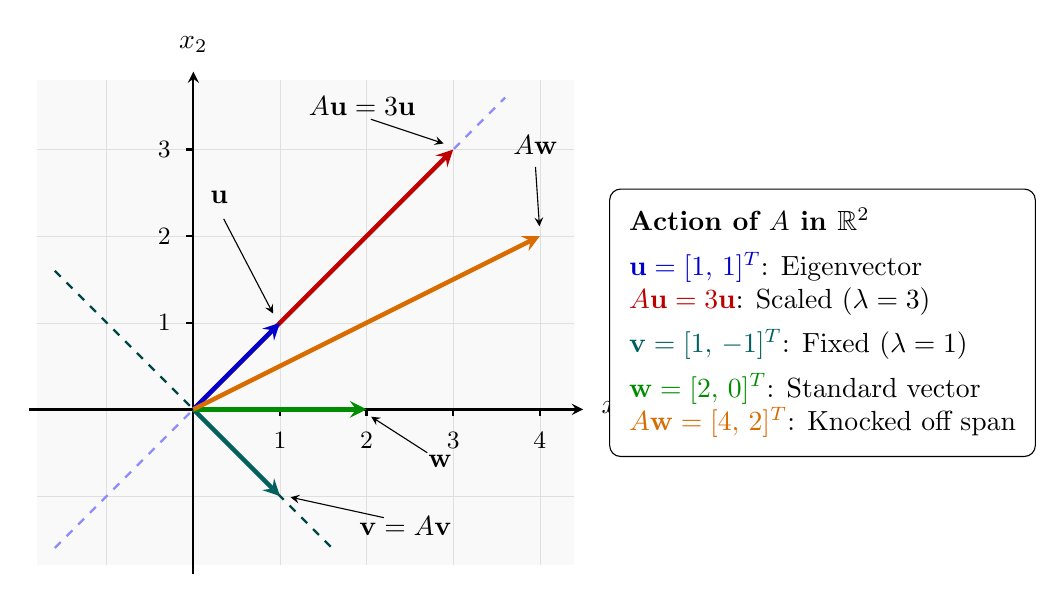
\begin{tikzpicture}[scale=1.1]
        % Layer 1: Background
        \fill[gray!5] (-1.8,-1.8) rectangle (4.4,3.8);

        % Layer 2: Grid and Axes
        \draw[step=1cm, gray!25, very thin] (-1.8,-1.8) grid (4.4,3.8);
        \draw[->, >=stealth, thick, black] (-1.9,0) -- (4.5,0) node[right=3pt, black] {$x_1$};
        \draw[->, >=stealth, thick, black] (0,-1.9) -- (0,3.9) node[above=3pt, black] {$x_2$};
        \foreach \x in {1,2,3,4}
            \draw[thick] (\x,0) -- (\x,-0.08) node[below=2pt, black] {\small $\x$};
        \foreach \y in {1,2,3}
            \draw[thick] (0,\y) -- (-0.08,\y) node[left=2pt, black] {\small $\y$};

        % Layer 3: Span Lines, Primary Vectors, and Callouts
        \draw[dashed, blue!45, thick] (-1.6,-1.6) -- (3.6,3.6);
        \draw[dashed, teal!55!black, thick] (-1.6,1.6) -- (1.6,-1.6);

        \draw[->, >=stealth, ultra thick, red!75!black] (0,0) -- (3,3);
        \draw[->, >=stealth, ultra thick, blue!80!black] (0,0) -- (1,1);
        \draw[->, >=stealth, ultra thick, teal!75!black] (0,0) -- (1,-1);
        \draw[->, >=stealth, ultra thick, green!55!black] (0,0) -- (2,0);
        \draw[->, >=stealth, ultra thick, orange!85!black] (0,0) -- (4,2);

        \draw[->, >=stealth, thin, shorten >=2pt] (0.35, 2.2) -- (0.95, 1.05);
        \draw[->, >=stealth, thin, shorten >=2pt] (2.05, 3.35) -- (2.95, 3.05);
        \draw[->, >=stealth, thin, shorten >=2pt] (2.2, -1.25) -- (1.06, -1.0);
        \draw[->, >=stealth, thin, shorten >=2pt] (2.7, -0.5) -- (2.0, -0.05);
        \draw[->, >=stealth, thin, shorten >=2pt] (3.95, 2.8) -- (4.0, 2.05);

        % Layer 4: Nodes and Single-Node Legend
        \node[black] at (0.3, 2.45) {$\mathbf{u}$};
        \node[black] at (1.95, 3.5) {$A\mathbf{u} = 3\mathbf{u}$};
        \node[black] at (2.45, -1.35) {$\mathbf{v} = A\mathbf{v}$};
        \node[black] at (2.85, -0.6) {$\mathbf{w}$};
        \node[black] at (3.95, 3.05) {$A\mathbf{w}$};

        \node[draw, rounded corners, fill=white, align=left, inner sep=7pt, anchor=west, text=black] at (4.8, 1.0) {
            \textbf{Action of $A$ in $\mathbb{R}^2$}\\[4pt]
            \textcolor{blue!80!black}{$\mathbf{u} = [1,\,1]^T$}: Eigenvector\\
            \textcolor{red!75!black}{$A\mathbf{u} = 3\mathbf{u}$}: Scaled ($\lambda = 3$)\\[4pt]
            \textcolor{teal!75!black}{$\mathbf{v} = [1,\,-1]^T$}: Fixed ($\lambda = 1$)\\[4pt]
            \textcolor{green!55!black}{$\mathbf{w} = [2,\,0]^T$}: Standard vector\\
            \textcolor{orange!85!black}{$A\mathbf{w} = [4,\,2]^T$}: Knocked off span
        };
    \end{tikzpicture}
    \end{center}
\end{enumerate}
\textbf{Final Answer:} $\mathbf{u}$ ($\lambda = 3$) and $\mathbf{v}$ ($\lambda = 1$) are eigenvectors; $\mathbf{w}$ (knocked off its span) and $\mathbf{z} = \mathbf{0}$ (zero vector) are not eigenvectors.

\vspace{0.4em}
\textbf{Problem 2:}
Determine whether $\mathbf{v} = \begin{bmatrix} 3 \\ -2 \end{bmatrix}$ is an eigenvector of $A = \begin{bmatrix} -1 & 3 \\ 2 & 0 \end{bmatrix}$. If it is, find the corresponding eigenvalue and describe the geometric effect of $A$ on $\mathbf{v}$.

\textbf{Solution:}
Compute $A\mathbf{v}$ directly:
\[
A\mathbf{v} = \begin{bmatrix} -1 & 3 \\ 2 & 0 \end{bmatrix}\begin{bmatrix} 3 \\ -2 \end{bmatrix} = \begin{bmatrix} -1(3) + 3(-2) \\ 2(3) + 0(-2) \end{bmatrix} = \begin{bmatrix} -9 \\ 6 \end{bmatrix} = -3\begin{bmatrix} 3 \\ -2 \end{bmatrix} = -3\mathbf{v}.
\]
Because $\mathbf{v} \neq \mathbf{0}$ and $A\mathbf{v} = \lambda\mathbf{v}$ holds consistently across both components for $\lambda = -3$, $\mathbf{v}$ is an eigenvector of $A$. Geometrically, multiplying by $A$ stretches $\mathbf{v}$ by a factor of $3$ while reversing its direction along the line $\operatorname{Span}\{\mathbf{v}\}$.

\textbf{Final Answer:} Yes, $\mathbf{v}$ is an eigenvector with eigenvalue $\lambda = -3$; $A$ stretches $\mathbf{v}$ by $3$ and flips its direction.

\vspace{0.4em}
\textbf{Problem 3:}
Consider the matrix and vectors
\[
A = \begin{bmatrix} 2 & -1 & 3 \\ 4 & -2 & 6 \\ -2 & 1 & 1 \end{bmatrix}, \quad \mathbf{v}_1 = \begin{bmatrix} 1 \\ 2 \\ 0 \end{bmatrix}, \quad \mathbf{v}_2 = \begin{bmatrix} 1 \\ 2 \\ 1 \end{bmatrix}.
\]
Determine whether $\mathbf{v}_1$ and $\mathbf{v}_2$ are eigenvectors of $A$. For each vector that is an eigenvector, determine its corresponding eigenvalue.

\textbf{Solution:}
First compute $A\mathbf{v}_1$:
\[
A\mathbf{v}_1 = \begin{bmatrix} 2 & -1 & 3 \\ 4 & -2 & 6 \\ -2 & 1 & 1 \end{bmatrix}\begin{bmatrix} 1 \\ 2 \\ 0 \end{bmatrix} = \begin{bmatrix} 2(1) - 1(2) + 3(0) \\ 4(1) - 2(2) + 6(0) \\ -2(1) + 1(2) + 1(0) \end{bmatrix} = \begin{bmatrix} 0 \\ 0 \\ 0 \end{bmatrix} = 0 \cdot \mathbf{v}_1.
\]
Because $\mathbf{v}_1 \neq \mathbf{0}$ and $A\mathbf{v}_1 = 0 \cdot \mathbf{v}_1$, $\mathbf{v}_1$ is an eigenvector with eigenvalue $\lambda = 0$.

Next compute $A\mathbf{v}_2$:
\[
A\mathbf{v}_2 = \begin{bmatrix} 2 & -1 & 3 \\ 4 & -2 & 6 \\ -2 & 1 & 1 \end{bmatrix}\begin{bmatrix} 1 \\ 2 \\ 1 \end{bmatrix} = \begin{bmatrix} 2 - 2 + 3 \\ 4 - 4 + 6 \\ -2 + 2 + 1 \end{bmatrix} = \begin{bmatrix} 3 \\ 6 \\ 1 \end{bmatrix}.
\]
Testing $A\mathbf{v}_2 = \lambda\mathbf{v}_2$ yields $\lambda = 3$ from the first two components ($3 = \lambda\cdot 1$ and $6 = \lambda\cdot 2$), but $\lambda = 1$ from the third component ($1 = \lambda\cdot 1$). Since no single scalar $\lambda$ satisfies all three equations simultaneously, $\mathbf{v}_2$ is not an eigenvector of $A$.

\textbf{Final Answer:} $\mathbf{v}_1$ is an eigenvector with $\lambda = 0$; $\mathbf{v}_2$ is not an eigenvector.

\vspace{0.4em}
\textbf{Problem 4:}
Is $\lambda = -3$ an eigenvalue of $A = \begin{bmatrix} -5 & 4 \\ -1 & -1 \end{bmatrix}$? Justify your answer rigorously using $(A - \lambda I)\mathbf{x} = \mathbf{0}$, and if yes, find one corresponding eigenvector.

\textbf{Solution:}
We test whether $(A - (-3)I)\mathbf{x} = (A + 3I)\mathbf{x} = \mathbf{0}$ has a nontrivial solution. Carefully subtracting $\lambda = -3$ from the negative diagonal entries gives:
\[
A + 3I = \begin{bmatrix} -5 - (-3) & 4 \\ -1 & -1 - (-3) \end{bmatrix} = \begin{bmatrix} -2 & 4 \\ -1 & 2 \end{bmatrix}.
\]
Row reduce the augmented matrix $\begin{bmatrix} -2 & 4 & 0 \\ -1 & 2 & 0 \end{bmatrix}$:
\begin{align*}
\begin{bmatrix} -2 & 4 & 0 \\ -1 & 2 & 0 \end{bmatrix} &\xrightarrow{R_1 \leftrightarrow R_2,\ R_1 \leftarrow -R_1} \begin{bmatrix} 1 & -2 & 0 \\ -2 & 4 & 0 \end{bmatrix} \\
&\xrightarrow{R_2 \leftarrow R_2 + 2R_1} \begin{bmatrix} 1 & -2 & 0 \\ 0 & 0 & 0 \end{bmatrix}.
\end{align*}
Since column $2$ lacks a pivot, $x_2$ is a free variable, confirming nontrivial solutions exist. The equation $x_1 - 2x_2 = 0$ gives $x_1 = 2x_2$. Choosing $x_2 = 1$ yields the eigenvector $\mathbf{v} = \begin{bmatrix} 2 \\ 1 \end{bmatrix}$. Verification: $A\mathbf{v} = \begin{bmatrix} -10 + 4 \\ -2 - 1 \end{bmatrix} = \begin{bmatrix} -6 \\ -3 \end{bmatrix} = -3\mathbf{v}$.

\textbf{Final Answer:} Yes, $\lambda = -3$ is an eigenvalue; one corresponding eigenvector is $\begin{bmatrix} 2 \\ 1 \end{bmatrix}$.

\vspace{0.4em}
\textbf{Problem 5:}
Determine whether $\lambda = 2$ and $\lambda = 5$ are eigenvalues of
\[
A = \begin{bmatrix} 4 & -1 & 2 \\ 1 & 2 & 1 \\ -2 & 2 & 0 \end{bmatrix}.
\]
For any value that is an eigenvalue, compute one corresponding eigenvector.

\textbf{Solution:}
\textbf{Case 1 ($\lambda = 2$):} Construct $A - 2I$ and row reduce the homogeneous augmented matrix:
\[
\begin{bmatrix} 2 & -1 & 2 & 0 \\ 1 & 0 & 1 & 0 \\ -2 & 2 & -2 & 0 \end{bmatrix}
\xrightarrow{R_1 \leftrightarrow R_2}
\begin{bmatrix} 1 & 0 & 1 & 0 \\ 2 & -1 & 2 & 0 \\ -2 & 2 & -2 & 0 \end{bmatrix}
\xrightarrow{\substack{R_2 \leftarrow R_2 - 2R_1 \\ R_3 \leftarrow R_3 + 2R_1}}
\begin{bmatrix} 1 & 0 & 1 & 0 \\ 0 & -1 & 0 & 0 \\ 0 & 2 & 0 & 0 \end{bmatrix}
\xrightarrow{\substack{R_3 \leftarrow R_3 + 2R_2 \\ R_2 \leftarrow -R_2}}
\begin{bmatrix} 1 & 0 & 1 & 0 \\ 0 & 1 & 0 & 0 \\ 0 & 0 & 0 & 0 \end{bmatrix}.
\]
Here $x_3$ is a free variable, so $(A - 2I)\mathbf{x} = \mathbf{0}$ has nontrivial solutions: $x_1 = -x_3$ and $x_2 = 0$. Setting $x_3 = 1$ produces the eigenvector $\mathbf{v} = \begin{bmatrix} -1 \\ 0 \\ 1 \end{bmatrix}$.

\textbf{Case 2 ($\lambda = 5$):} Construct $A - 5I$ and row reduce:
\[
\begin{bmatrix} -1 & -1 & 2 & 0 \\ 1 & -3 & 1 & 0 \\ -2 & 2 & -5 & 0 \end{bmatrix}
\xrightarrow{R_1 \leftarrow -R_1}
\begin{bmatrix} 1 & 1 & -2 & 0 \\ 1 & -3 & 1 & 0 \\ -2 & 2 & -5 & 0 \end{bmatrix}
\xrightarrow{\substack{R_2 \leftarrow R_2 - R_1 \\ R_3 \leftarrow R_3 + 2R_1}}
\begin{bmatrix} 1 & 1 & -2 & 0 \\ 0 & -4 & 3 & 0 \\ 0 & 4 & -9 & 0 \end{bmatrix}
\xrightarrow{R_3 \leftarrow R_3 + R_2}
\begin{bmatrix} 1 & 1 & -2 & 0 \\ 0 & -4 & 3 & 0 \\ 0 & 0 & -6 & 0 \end{bmatrix}.
\]
There is a pivot in every variable column (all three columns), so there are no free variables and the only solution to $(A - 5I)\mathbf{x} = \mathbf{0}$ is $\mathbf{x} = \mathbf{0}$. Thus $\lambda = 5$ is not an eigenvalue.

\textbf{Final Answer:} $\lambda = 2$ is an eigenvalue with eigenvector $\begin{bmatrix} -1 \\ 0 \\ 1 \end{bmatrix}$; $\lambda = 5$ is not an eigenvalue.

\subsection{Eigenspace Extraction, Triangular Shortcuts, and Zero Eigenvalues (Problems 6--12)}

\textbf{Problem 6:}
Find a basis for each eigenspace of $A = \begin{bmatrix} 5 & -2 \\ -4 & 7 \end{bmatrix}$ corresponding to the eigenvalues $\lambda = 3$ and $\lambda = 9$.

\textbf{Solution:}
\textbf{For $\lambda = 3$:}
\[
A - 3I = \begin{bmatrix} 2 & -2 \\ -4 & 4 \end{bmatrix} \sim \begin{bmatrix} 1 & -1 \\ 0 & 0 \end{bmatrix}.
\]
This gives $x_1 = x_2$ with $x_2$ free, so $\mathbf{x} = x_2 \begin{bmatrix} 1 \\ 1 \end{bmatrix}$. Basis for $E_3$: $\left\{ \begin{bmatrix} 1 \\ 1 \end{bmatrix} \right\}$.

\textbf{For $\lambda = 9$:}
\[
A - 9I = \begin{bmatrix} -4 & -2 \\ -4 & -2 \end{bmatrix} \sim \begin{bmatrix} 2 & 1 \\ 0 & 0 \end{bmatrix} \sim \begin{bmatrix} 1 & 1/2 \\ 0 & 0 \end{bmatrix}.
\]
This gives $x_1 = -\frac{1}{2}x_2$ with $x_2$ free. Clearing the fraction by setting $x_2 = 2$ gives $\begin{bmatrix} -1 \\ 2 \end{bmatrix}$. Basis for $E_9$: $\left\{ \begin{bmatrix} -1 \\ 2 \end{bmatrix} \right\}$.

\textbf{Final Answer:} Basis for $\lambda = 3$ is $\left\{ \begin{bmatrix} 1 \\ 1 \end{bmatrix} \right\}$; basis for $\lambda = 9$ is $\left\{ \begin{bmatrix} -1 \\ 2 \end{bmatrix} \right\}$.

\vspace{0.4em}
\textbf{Problem 7:}
Find a basis for the eigenspaces of
\[
A = \begin{bmatrix} -1 & 6 & 0 \\ 3 & 5 & -3 \\ -3 & 6 & 2 \end{bmatrix}
\]
corresponding to the eigenvalues $\lambda = -1, 2, 5$. Express each basis vector with integer entries by clearing fractions where appropriate.

\textbf{Solution:}
\textbf{For $\lambda = -1$:}
\[
A + I = \begin{bmatrix} 0 & 6 & 0 \\ 3 & 6 & -3 \\ -3 & 6 & 3 \end{bmatrix}
\xrightarrow{\substack{R_1 \leftarrow \frac{1}{6}R_1 \\ R_2 \leftarrow \frac{1}{3}R_2}}
\begin{bmatrix} 0 & 1 & 0 \\ 1 & 2 & -1 \\ -3 & 6 & 3 \end{bmatrix}
\sim
\begin{bmatrix} 1 & 0 & -1 \\ 0 & 1 & 0 \\ 0 & 0 & 0 \end{bmatrix}.
\]
Hence $x_1 = x_3$, $x_2 = 0$, and $x_3$ is free, giving basis $\left\{ \begin{bmatrix} 1 \\ 0 \\ 1 \end{bmatrix} \right\}$.

\textbf{For $\lambda = 2$:}
\[
A - 2I = \begin{bmatrix} -3 & 6 & 0 \\ 3 & 3 & -3 \\ -3 & 6 & 0 \end{bmatrix}
\xrightarrow{\substack{R_3 \leftarrow R_3 - R_1 \\ R_2 \leftarrow R_2 + R_1 \\ R_1 \leftarrow -\frac{1}{3}R_1}}
\begin{bmatrix} 1 & -2 & 0 \\ 0 & 9 & -3 \\ 0 & 0 & 0 \end{bmatrix}
\xrightarrow{\substack{R_2 \leftarrow \frac{1}{9}R_2 \\ R_1 \leftarrow R_1 + 2R_2}}
\begin{bmatrix} 1 & 0 & -2/3 \\ 0 & 1 & -1/3 \\ 0 & 0 & 0 \end{bmatrix}.
\]
Thus $x_1 = \frac{2}{3}x_3$, $x_2 = \frac{1}{3}x_3$, and $x_3$ is free. Setting $x_3 = 3$ clears all denominators and gives the integer basis $\left\{ \begin{bmatrix} 2 \\ 1 \\ 3 \end{bmatrix} \right\}$.

\textbf{For $\lambda = 5$:}
\[
A - 5I = \begin{bmatrix} -6 & 6 & 0 \\ 3 & 0 & -3 \\ -3 & 6 & -3 \end{bmatrix}
\xrightarrow{\substack{R_1 \leftarrow -\frac{1}{6}R_1 \\ R_2 \leftarrow \frac{1}{3}R_2}}
\begin{bmatrix} 1 & -1 & 0 \\ 1 & 0 & -1 \\ -3 & 6 & -3 \end{bmatrix}
\sim
\begin{bmatrix} 1 & 0 & -1 \\ 0 & 1 & -1 \\ 0 & 0 & 0 \end{bmatrix}.
\]
Thus $x_1 = x_3$, $x_2 = x_3$, and $x_3$ is free, giving basis $\left\{ \begin{bmatrix} 1 \\ 1 \\ 1 \end{bmatrix} \right\}$.

\textbf{Final Answer:} Bases are $\left\{ \begin{bmatrix} 1 \\ 0 \\ 1 \end{bmatrix} \right\}$ ($\lambda = -1$), $\left\{ \begin{bmatrix} 2 \\ 1 \\ 3 \end{bmatrix} \right\}$ ($\lambda = 2$), and $\left\{ \begin{bmatrix} 1 \\ 1 \\ 1 \end{bmatrix} \right\}$ ($\lambda = 5$).

\vspace{0.4em}
\textbf{Problem 8:}
Find a basis for each eigenspace of
\[
B = \begin{bmatrix} 6 & -2 & 2 \\ -2 & 3 & -1 \\ 2 & -1 & 3 \end{bmatrix}
\]
corresponding to $\lambda = 2$ and $\lambda = 8$, and state the geometric dimension of each eigenspace in $\mathbb{R}^3$.

\textbf{Solution:}
\textbf{For $\lambda = 2$:}
\[
B - 2I = \begin{bmatrix} 4 & -2 & 2 \\ -2 & 1 & -1 \\ 2 & -1 & 1 \end{bmatrix}
\xrightarrow{\substack{R_1 \leftarrow \frac{1}{4}R_1 \\ R_2 \leftarrow R_2 + 2R_1 \\ R_3 \leftarrow R_3 - 2R_1}}
\begin{bmatrix} 1 & -1/2 & 1/2 \\ 0 & 0 & 0 \\ 0 & 0 & 0 \end{bmatrix}.
\]
Here there are two free variables, $x_2$ and $x_3$, with $x_1 = \frac{1}{2}x_2 - \frac{1}{2}x_3$. Writing in parametric vector form:
\[
\mathbf{x} = x_2 \begin{bmatrix} 1/2 \\ 1 \\ 0 \end{bmatrix} + x_3 \begin{bmatrix} -1/2 \\ 0 \\ 1 \end{bmatrix}.
\]
Scaling each basis vector by $2$ to clear fractions yields the basis $\left\{ \begin{bmatrix} 1 \\ 2 \\ 0 \end{bmatrix}, \begin{bmatrix} -1 \\ 0 \\ 2 \end{bmatrix} \right\}$. Since there are $2$ linearly independent basis vectors, $E_2$ is a $2$-dimensional plane in $\mathbb{R}^3$.

\textbf{For $\lambda = 8$:}
\[
B - 8I = \begin{bmatrix} -2 & -2 & 2 \\ -2 & -5 & -1 \\ 2 & -1 & -5 \end{bmatrix}
\xrightarrow{\substack{R_2 \leftarrow R_2 - R_1 \\ R_3 \leftarrow R_3 + R_1 \\ R_1 \leftarrow -\frac{1}{2}R_1}}
\begin{bmatrix} 1 & 1 & -1 \\ 0 & -3 & -3 \\ 0 & -3 & -3 \end{bmatrix}
\sim
\begin{bmatrix} 1 & 0 & -2 \\ 0 & 1 & 1 \\ 0 & 0 & 0 \end{bmatrix}.
\]
Thus $x_1 = 2x_3$, $x_2 = -x_3$, and $x_3$ is free, giving basis $\left\{ \begin{bmatrix} 2 \\ -1 \\ 1 \end{bmatrix} \right\}$, which is a $1$-dimensional line in $\mathbb{R}^3$.

\textbf{Final Answer:} $E_2$ has basis $\left\{ \begin{bmatrix} 1 \\ 2 \\ 0 \end{bmatrix}, \begin{bmatrix} -1 \\ 0 \\ 2 \end{bmatrix} \right\}$ (dimension $2$); $E_8$ has basis $\left\{ \begin{bmatrix} 2 \\ -1 \\ 1 \end{bmatrix} \right\}$ (dimension $1$).

\vspace{0.4em}
\textbf{Problem 9:}
Find a basis for the eigenspace of
\[
A = \begin{bmatrix} 4 & -3 & 2 \\ 0 & 5 & -1 \\ 0 & 0 & 4 \end{bmatrix}
\]
corresponding to $\lambda = 4$, carefully tracking all pivot columns and free variables in the Reduced Row Echelon Form (RREF).

\textbf{Solution:}
Construct $A - 4I$:
\[
A - 4I = \begin{bmatrix} 0 & -3 & 2 \\ 0 & 1 & -1 \\ 0 & 0 & 0 \end{bmatrix}.
\]
Notice that column $1$ consists entirely of zeros; therefore, $x_1$ has no pivot and is a free variable. We row reduce columns $2$ and $3$ to RREF:
\[
\begin{bmatrix} 0 & -3 & 2 \\ 0 & 1 & -1 \\ 0 & 0 & 0 \end{bmatrix}
\xrightarrow{R_1 \leftrightarrow R_2}
\begin{bmatrix} 0 & 1 & -1 \\ 0 & -3 & 2 \\ 0 & 0 & 0 \end{bmatrix}
\xrightarrow{R_2 \leftarrow R_2 + 3R_1}
\begin{bmatrix} 0 & 1 & -1 \\ 0 & 0 & -1 \\ 0 & 0 & 0 \end{bmatrix}
\xrightarrow{\substack{R_2 \leftarrow -R_2 \\ R_1 \leftarrow R_1 + R_2}}
\begin{bmatrix} 0 & 1 & 0 \\ 0 & 0 & 1 \\ 0 & 0 & 0 \end{bmatrix}.
\]
The pivot columns are columns $2$ and $3$, giving $x_2 = 0$ and $x_3 = 0$, while $x_1$ remains free. The parametric vector form of the solution is
\[
\mathbf{x} = \begin{bmatrix} x_1 \\ 0 \\ 0 \end{bmatrix} = x_1 \begin{bmatrix} 1 \\ 0 \\ 0 \end{bmatrix}.
\]
Verification: $A\begin{bmatrix} 1 \\ 0 \\ 0 \end{bmatrix} = \begin{bmatrix} 4 \\ 0 \\ 0 \end{bmatrix} = 4\begin{bmatrix} 1 \\ 0 \\ 0 \end{bmatrix}$.

\textbf{Final Answer:} A basis for the eigenspace corresponding to $\lambda = 4$ is $\left\{ \begin{bmatrix} 1 \\ 0 \\ 0 \end{bmatrix} \right\}$.

\vspace{0.4em}
\textbf{Problem 10:}
Consider the $4 \times 4$ matrix
\[
A = \begin{bmatrix} -2 & 0 & 0 & 0 \\ 7 & 5 & 0 & 0 \\ -3 & 4 & 5 & 0 \\ 9 & -1 & 6 & 0 \end{bmatrix}.
\]
\begin{enumerate}[label=(\alph*)]
    \item Without computing cofactor expansions or row-reducing $A$, state all eigenvalues of $A$ and justify your answer.
    \item Determine whether $A$ is invertible based solely on your answer to part (a).
    \item Find a basis for the eigenspace corresponding to $\lambda = 5$.
\end{enumerate}

\textbf{Solution:}
\begin{enumerate}[label=(\alph*)]
    \item Because all entries strictly above the main diagonal are zero, $A$ is a lower-triangular matrix. By the Triangular Matrix Theorem, the eigenvalues of a triangular matrix are precisely the entries on its main diagonal. Hence the distinct eigenvalues of $A$ are $\lambda = -2, 5, 0$ (with $5$ appearing twice on the diagonal).

    \item Since $\lambda = 0$ is an eigenvalue of $A$, the homogeneous equation $(A - 0I)\mathbf{x} = A\mathbf{x} = \mathbf{0}$ has a nontrivial solution. Equivalently, $\operatorname{Nul}(A) \neq \{\mathbf{0}\}$, so $A$ is \emph{not} invertible.

    \item Construct $A - 5I$ and row reduce to RREF:
    \begin{align*}
    A - 5I &= \begin{bmatrix} -7 & 0 & 0 & 0 \\ 7 & 0 & 0 & 0 \\ -3 & 4 & 0 & 0 \\ 9 & -1 & 6 & -5 \end{bmatrix}
    \xrightarrow{\substack{R_1 \leftarrow -\frac{1}{7}R_1 \\ R_2 \leftarrow R_2 - 7R_1 \\ R_3 \leftarrow R_3 + 3R_1 \\ R_4 \leftarrow R_4 - 9R_1}}
    \begin{bmatrix} 1 & 0 & 0 & 0 \\ 0 & 0 & 0 & 0 \\ 0 & 4 & 0 & 0 \\ 0 & -1 & 6 & -5 \end{bmatrix} \\
    &\xrightarrow{\substack{R_2 \leftrightarrow R_3,\ R_2 \leftarrow \frac{1}{4}R_2 \\ R_4 \leftarrow R_4 + R_2 \\ R_3 \leftrightarrow R_4,\ R_3 \leftarrow \frac{1}{6}R_3}}
    \begin{bmatrix} 1 & 0 & 0 & 0 \\ 0 & 1 & 0 & 0 \\ 0 & 0 & 1 & -5/6 \\ 0 & 0 & 0 & 0 \end{bmatrix}.
    \end{align*}
    The equations are $x_1 = 0$, $x_2 = 0$, and $x_3 = \frac{5}{6}x_4$, with $x_4$ free. Choosing $x_4 = 6$ to clear the fraction gives $\begin{bmatrix} 0 \\ 0 \\ 5 \\ 6 \end{bmatrix}$.
\end{enumerate}
\textbf{Final Answer:} (a) $\lambda = -2, 5, 0$; (b) $A$ is not invertible; (c) basis for $E_5$ is $\left\{ \begin{bmatrix} 0 \\ 0 \\ 5 \\ 6 \end{bmatrix} \right\}$.

\vspace{0.4em}
\textbf{Problem 11:}
Let $k \in \mathbb{R}$ and consider the matrix
\[
A = \begin{bmatrix} 1 & 2 & -1 \\ 3 & 5 & -1 \\ 2 & k & 4 \end{bmatrix}.
\]
\begin{enumerate}[label=(\alph*)]
    \item Find the exact value of $k$ for which $\lambda = 0$ is an eigenvalue of $A$.
    \item For that value of $k$, find a basis for the eigenspace corresponding to $\lambda = 0$ and explain how this result relates to the invertibility of $A$.
\end{enumerate}

\textbf{Solution:}
\begin{enumerate}[label=(\alph*)]
    \item The scalar $\lambda = 0$ is an eigenvalue of $A$ if and only if $(A - 0I)\mathbf{x} = A\mathbf{x} = \mathbf{0}$ has a nontrivial solution, which occurs if and only if $A$ has a row of zeros in echelon form (equivalently, $\det(A) = 0$). Row reduce $A$:
    \begin{align*}
    \begin{bmatrix} 1 & 2 & -1 \\ 3 & 5 & -1 \\ 2 & k & 4 \end{bmatrix}
    &\xrightarrow{\substack{R_2 \leftarrow R_2 - 3R_1 \\ R_3 \leftarrow R_3 - 2R_1}}
    \begin{bmatrix} 1 & 2 & -1 \\ 0 & -1 & 2 \\ 0 & k-4 & 6 \end{bmatrix} \\
    &\xrightarrow{R_2 \leftarrow -R_2}
    \begin{bmatrix} 1 & 2 & -1 \\ 0 & 1 & -2 \\ 0 & k-4 & 6 \end{bmatrix}
    \xrightarrow{R_3 \leftarrow R_3 - (k-4)R_2}
    \begin{bmatrix} 1 & 2 & -1 \\ 0 & 1 & -2 \\ 0 & 0 & 2k - 2 \end{bmatrix}.
    \end{align*}
    The third pivot vanishes (creating a free variable $x_3$) if and only if $2k - 2 = 0$, which yields $k = 1$. (Confirming via determinant: $\det(A) = 1(20+k) - 2(12+2) - 1(3k-10) = 2 - 2k = 0 \iff k = 1$.)

    \item Setting $k = 1$ in the echelon form and reducing to RREF gives:
    \[
    \begin{bmatrix} 1 & 2 & -1 \\ 0 & 1 & -2 \\ 0 & 0 & 0 \end{bmatrix}
    \xrightarrow{R_1 \leftarrow R_1 - 2R_2}
    \begin{bmatrix} 1 & 0 & 3 \\ 0 & 1 & -2 \\ 0 & 0 & 0 \end{bmatrix}.
    \]
    Hence $x_1 = -3x_3$ and $x_2 = 2x_3$, with $x_3$ free, giving the basis $\left\{ \begin{bmatrix} -3 \\ 2 \\ 1 \end{bmatrix} \right\}$ for $E_0 = \operatorname{Nul}(A)$. Because $\lambda = 0$ is an eigenvalue of $A$ when $k = 1$, $\operatorname{Nul}(A)$ is nontrivial and $\det(A) = 0$, meaning $A$ is singular (not invertible) precisely at $k = 1$.
\end{enumerate}
\textbf{Final Answer:} (a) $k = 1$; (b) basis for $E_0$ is $\left\{ \begin{bmatrix} -3 \\ 2 \\ 1 \end{bmatrix} \right\}$, and $A$ fails to be invertible at $k = 1$ because $0$ is an eigenvalue.

\vspace{0.4em}
\textbf{Problem 12:}
Using the characteristic equation $\det(A - \lambda I) = 0$, find all eigenvalues and a basis for each corresponding eigenspace of
\[
A = \begin{bmatrix} 2 & 1 & 1 \\ 0 & 4 & 0 \\ 3 & -1 & 0 \end{bmatrix}.
\]

\textbf{Solution:}
Compute the characteristic polynomial by expanding along the second row (which has two zeros):
\begin{align*}
\det(A - \lambda I) &= \det \begin{bmatrix} 2 - \lambda & 1 & 1 \\ 0 & 4 - \lambda & 0 \\ 3 & -1 & -\lambda \end{bmatrix} \\
&= (4 - \lambda)\bigl[(2 - \lambda)(-\lambda) - (1)(3)\bigr] \\
&= (4 - \lambda)(\lambda^2 - 2\lambda - 3) \\
&= (4 - \lambda)(\lambda - 3)(\lambda + 1) = 0.
\end{align*}
Thus the eigenvalues of $A$ are $\lambda = -1, 3, 4$.

\textbf{For $\lambda = -1$:}
\[
A + I = \begin{bmatrix} 3 & 1 & 1 \\ 0 & 5 & 0 \\ 3 & -1 & 1 \end{bmatrix}
\xrightarrow{\substack{R_2 \leftarrow \frac{1}{5}R_2 \\ R_1 \leftarrow R_1 - R_2 \\ R_3 \leftarrow R_3 + R_2}}
\begin{bmatrix} 3 & 0 & 1 \\ 0 & 1 & 0 \\ 3 & 0 & 1 \end{bmatrix}
\sim
\begin{bmatrix} 1 & 0 & 1/3 \\ 0 & 1 & 0 \\ 0 & 0 & 0 \end{bmatrix}.
\]
Hence $x_1 = -\frac{1}{3}x_3$, $x_2 = 0$, and $x_3$ is free. Setting $x_3 = 3$ clears fractions and gives basis $\left\{ \begin{bmatrix} -1 \\ 0 \\ 3 \end{bmatrix} \right\}$.

\textbf{For $\lambda = 3$:}
\[
A - 3I = \begin{bmatrix} -1 & 1 & 1 \\ 0 & 1 & 0 \\ 3 & -1 & -3 \end{bmatrix}
\xrightarrow{\substack{R_1 \leftarrow R_1 - R_2 \\ R_3 \leftarrow R_3 + R_2}}
\begin{bmatrix} -1 & 0 & 1 \\ 0 & 1 & 0 \\ 3 & 0 & -3 \end{bmatrix}
\sim
\begin{bmatrix} 1 & 0 & -1 \\ 0 & 1 & 0 \\ 0 & 0 & 0 \end{bmatrix}.
\]
Hence $x_1 = x_3$, $x_2 = 0$, and $x_3$ is free, giving basis $\left\{ \begin{bmatrix} 1 \\ 0 \\ 1 \end{bmatrix} \right\}$.

\textbf{For $\lambda = 4$:}
\[
A - 4I = \begin{bmatrix} -2 & 1 & 1 \\ 0 & 0 & 0 \\ 3 & -1 & -4 \end{bmatrix}
\xrightarrow{R_2 \leftrightarrow R_3}
\begin{bmatrix} -2 & 1 & 1 \\ 3 & -1 & -4 \\ 0 & 0 & 0 \end{bmatrix}
\xrightarrow{\substack{R_1 \leftarrow R_1 + R_2 \\ R_2 \leftarrow R_2 - 3R_1 \\ R_2 \leftarrow -R_2}}
\begin{bmatrix} 1 & 0 & -3 \\ 0 & 1 & -5 \\ 0 & 0 & 0 \end{bmatrix}.
\]
Hence $x_1 = 3x_3$, $x_2 = 5x_3$, and $x_3$ is free, giving basis $\left\{ \begin{bmatrix} 3 \\ 5 \\ 1 \end{bmatrix} \right\}$.

\textbf{Final Answer:} Eigenvalues $\lambda = -1, 3, 4$, with respective bases $\left\{ \begin{bmatrix} -1 \\ 0 \\ 3 \end{bmatrix} \right\}$, $\left\{ \begin{bmatrix} 1 \\ 0 \\ 1 \end{bmatrix} \right\}$, and $\left\{ \begin{bmatrix} 3 \\ 5 \\ 1 \end{bmatrix} \right\}$.

\subsection{Complex Eigenvalues and Multiplicity Analysis (Problems 13--18)}

\textbf{Problem 13:}
Consider the matrix $A = \begin{bmatrix} 3 & -4 \\ 4 & 3 \end{bmatrix}$.
\begin{enumerate}[label=(\alph*)]
    \item Find all eigenvalues of $A$ over $\mathbb{C}$.
    \item Explain geometrically why $A$ possesses no real eigenvectors in $\mathbb{R}^2$.
    \item Find a basis over $\mathbb{C}$ for the eigenspace corresponding to the eigenvalue with positive imaginary part.
\end{enumerate}

\textbf{Solution:}
\begin{enumerate}[label=(\alph*)]
    \item Solve the characteristic equation $\det(A - \lambda I) = 0$:
    \[
    \det \begin{bmatrix} 3 - \lambda & -4 \\ 4 & 3 - \lambda \end{bmatrix} = (3 - \lambda)^2 + 16 = 0 \implies (3 - \lambda)^2 = -16 \implies 3 - \lambda = \pm 4i.
    \]
    Therefore, the complex eigenvalues are $\lambda = 3 + 4i$ and $\lambda = 3 - 4i$.

    \item Factoring out $5 = \sqrt{3^2 + 4^2}$ writes $A$ in rotation-scaling form:
    \[
    A = 5 \begin{bmatrix} 3/5 & -4/5 \\ 4/5 & 3/5 \end{bmatrix} = 5 \begin{bmatrix} \cos\theta & -\sin\theta \\ \sin\theta & \cos\theta \end{bmatrix}, \quad \text{where } \theta = \arccos(3/5) \approx 53.13^\circ.
    \]
    Geometrically, $A$ rotates every nonzero vector in $\mathbb{R}^2$ counterclockwise by $\theta \approx 53.13^\circ$ while scaling its length by $5$. Since $\theta$ is not an integer multiple of $180^\circ$, no nonzero real vector stays on its original span line, so no real eigenvectors exist.

    \item For $\lambda = 3 + 4i$:
    \[
    A - (3 + 4i)I = \begin{bmatrix} -4i & -4 \\ 4 & -4i \end{bmatrix}.
    \]
    Notice that $R_2 = i R_1$ because $i(-4i) = 4$ and $i(-4) = -4i$. Dividing $R_1$ by $-4$ and eliminating $R_2$ gives
    \[
    \begin{bmatrix} i & 1 \\ 0 & 0 \end{bmatrix} \xrightarrow{R_1 \leftarrow -i R_1} \begin{bmatrix} 1 & -i \\ 0 & 0 \end{bmatrix}.
    \]
    Thus $x_1 = i x_2$ with $x_2$ free (equivalently $x_2 = -i x_1$ with $x_1 = 1$). Choosing $x_1 = 1$ yields the basis $\left\{ \begin{bmatrix} 1 \\ -i \end{bmatrix} \right\}$ (equivalently $\left\{ \begin{bmatrix} i \\ 1 \end{bmatrix} \right\}$).
\end{enumerate}
\textbf{Final Answer:} (a) $\lambda = 3 \pm 4i$; (b) $A$ combines scaling by $5$ with rotation by $\arccos(3/5) \not\equiv 0 \pmod{\pi}$, leaving no real span invariant; (c) $\left\{ \begin{bmatrix} 1 \\ -i \end{bmatrix} \right\}$.

\vspace{0.4em}
\textbf{Problem 14:}
Let $R_\theta = \begin{bmatrix} \cos\theta & -\sin\theta \\ \sin\theta & \cos\theta \end{bmatrix}$ represent a counterclockwise rotation in $\mathbb{R}^2$ by an angle $\theta \in (0, \pi)$.
\begin{enumerate}[label=(\alph*)]
    \item Compute the characteristic polynomial of $R_\theta$ and prove algebraically that $R_\theta$ has no real eigenvalues for $\theta \in (0, \pi)$.
    \item Find the complex eigenvalues of $R_\theta$ in both trigonometric and polar exponential form ($e^{\pm i\theta}$), and determine a complex eigenvector for each eigenvalue.
\end{enumerate}

\textbf{Solution:}
\begin{enumerate}[label=(\alph*)]
    \item Compute the characteristic polynomial:
    \begin{align*}
    \det(R_\theta - \lambda I) &= (\cos\theta - \lambda)^2 + \sin^2\theta \\
    &= \lambda^2 - 2(\cos\theta)\lambda + (\cos^2\theta + \sin^2\theta) \\
    &= \lambda^2 - 2(\cos\theta)\lambda + 1.
    \end{align*}
    The quadratic discriminant is
    \[
    \Delta = (-2\cos\theta)^2 - 4(1)(1) = 4(\cos^2\theta - 1) = -4\sin^2\theta.
    \]
    For every $\theta \in (0, \pi)$, $\sin\theta > 0$, so $\Delta = -4\sin^2\theta < 0$. Because the discriminant is strictly negative, the characteristic equation has no real roots, proving $R_\theta$ has no real eigenvalues.

    \begin{center}
    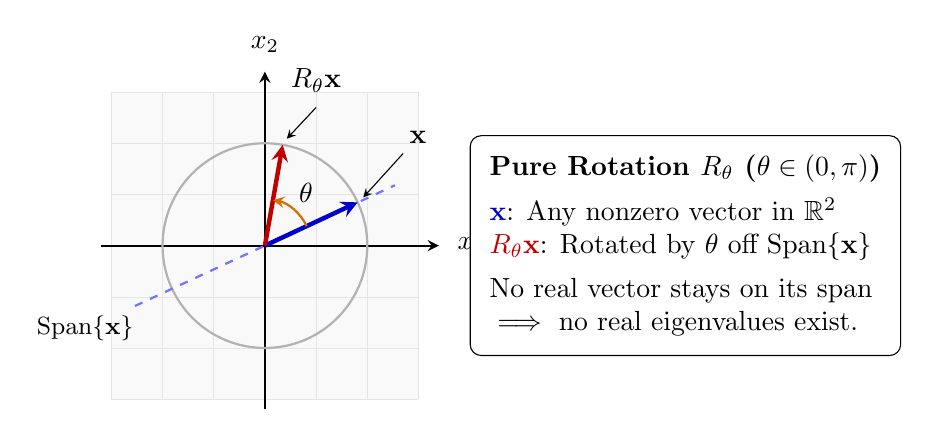
\begin{tikzpicture}[scale=1.3]
        % Layer 1: Background
        \fill[gray!5] (-1.5,-1.5) rectangle (1.5,1.5);

        % Layer 2: Grid and Axes
        \draw[step=0.5cm, gray!20, very thin] (-1.5,-1.5) grid (1.5,1.5);
        \draw[->, >=stealth, thick, black] (-1.6,0) -- (1.7,0) node[right=3pt, black] {$x_1$};
        \draw[->, >=stealth, thick, black] (0,-1.6) -- (0,1.7) node[above=3pt, black] {$x_2$};

        % Layer 3: Circle, Span Line, Vectors, Arc, and Callouts
        \draw[gray!60, thick] (0,0) circle (1);
        \draw[dashed, blue!55, thick] (-1.27,-0.59) -- (1.27,0.59);
        \draw[->, >=stealth, ultra thick, blue!80!black] (0,0) -- (25:1);
        \draw[->, >=stealth, ultra thick, red!75!black] (0,0) -- (80:1);
        \draw[->, >=stealth, thick, orange!85!black] (25:0.45) arc (25:80:0.45);

        \draw[->, >=stealth, thin, shorten >=2pt] (1.35, 0.9) -- (25:1.02);
        \draw[->, >=stealth, thin, shorten >=2pt] (0.5, 1.35) -- (80:1.02);

        % Layer 4: Labels and Single-Node Legend
        \node[black] at (52:0.65) {$\theta$};
        \node[above right=1pt, black] at (1.30, 0.88) {$\mathbf{x}$};
        \node[above=2pt, black] at (0.5, 1.35) {$R_\theta \mathbf{x}$};
        \node[below left=2pt, black] at (-1.15, -0.55) {\small $\operatorname{Span}\{\mathbf{x}\}$};

        \node[draw, rounded corners, fill=white, align=left, inner sep=7pt, anchor=west, text=black] at (2.0, 0.0) {
            \textbf{Pure Rotation $R_\theta$ ($\theta \in (0,\pi)$)}\\[4pt]
            \textcolor{blue!80!black}{$\mathbf{x}$}: Any nonzero vector in $\mathbb{R}^2$\\
            \textcolor{red!75!black}{$R_\theta \mathbf{x}$}: Rotated by $\theta$ off $\operatorname{Span}\{\mathbf{x}\}$\\[4pt]
            No real vector stays on its span\\
            $\implies$ no real eigenvalues exist.
        };
    \end{tikzpicture}
    \end{center}

    \item Applying the quadratic formula over $\mathbb{C}$ gives
    \[
    \lambda = \frac{2\cos\theta \pm \sqrt{-4\sin^2\theta}}{2} = \cos\theta \pm i\sin\theta = e^{\pm i\theta}.
    \]
    For $\lambda_1 = \cos\theta + i\sin\theta = e^{i\theta}$:
    \[
    R_\theta - \lambda_1 I = \begin{bmatrix} -i\sin\theta & -\sin\theta \\ \sin\theta & -i\sin\theta \end{bmatrix}.
    \]
    Since $\sin\theta \neq 0$, dividing the first row by $-\sin\theta$ yields $i x_1 + x_2 = 0 \implies x_2 = -i x_1$. (The second row is $i$ times the first row.) Setting $x_1 = 1$ gives $\mathbf{v}_1 = \begin{bmatrix} 1 \\ -i \end{bmatrix}$.

    For $\lambda_2 = \cos\theta - i\sin\theta = e^{-i\theta}$, conjugating (or solving $R_\theta - \lambda_2 I$) yields $-i x_1 + x_2 = 0 \implies x_2 = i x_1$, giving $\mathbf{v}_2 = \begin{bmatrix} 1 \\ i \end{bmatrix}$.
\end{enumerate}
\textbf{Final Answer:} (a) $\lambda^2 - 2(\cos\theta)\lambda + 1$ with $\Delta = -4\sin^2\theta < 0$; (b) $\lambda_1 = e^{i\theta}$ with $\mathbf{v}_1 = \begin{bmatrix} 1 \\ -i \end{bmatrix}$, and $\lambda_2 = e^{-i\theta}$ with $\mathbf{v}_2 = \begin{bmatrix} 1 \\ i \end{bmatrix}$.

\vspace{0.4em}
\textbf{Problem 15:}
Consider the $3 \times 3$ matrix
\[
A = \begin{bmatrix} 2 & 0 & 0 \\ 1 & 1 & -2 \\ 0 & 2 & 1 \end{bmatrix}.
\]
Find all real and complex eigenvalues of $A$, and find a basis for the real eigenspace corresponding to the real eigenvalue.

\textbf{Solution:}
Expand $\det(A - \lambda I)$ along the first row:
\[
\det(A - \lambda I) = (2 - \lambda)\det \begin{bmatrix} 1 - \lambda & -2 \\ 2 & 1 - \lambda \end{bmatrix} = (2 - \lambda)\bigl[(1 - \lambda)^2 + 4\bigr] = 0.
\]
Setting each factor to zero yields $\lambda_1 = 2$, and $(1 - \lambda)^2 = -4 \implies 1 - \lambda = \pm 2i \implies \lambda = 1 \pm 2i$. Thus the eigenvalues are $\lambda_1 = 2$ (real) and $\lambda_{2,3} = 1 \pm 2i$ (complex conjugates).

For the real eigenvalue $\lambda_1 = 2$, construct $A - 2I$ and row reduce:
\[
A - 2I = \begin{bmatrix} 0 & 0 & 0 \\ 1 & -1 & -2 \\ 0 & 2 & -1 \end{bmatrix}
\xrightarrow{\substack{R_1 \leftrightarrow R_2 \\ R_2 \leftrightarrow R_3}}
\begin{bmatrix} 1 & -1 & -2 \\ 0 & 2 & -1 \\ 0 & 0 & 0 \end{bmatrix}
\xrightarrow{\substack{R_2 \leftarrow \frac{1}{2}R_2 \\ R_1 \leftarrow R_1 + R_2}}
\begin{bmatrix} 1 & 0 & -5/2 \\ 0 & 1 & -1/2 \\ 0 & 0 & 0 \end{bmatrix}.
\]
Hence $x_1 = \frac{5}{2}x_3$ and $x_2 = \frac{1}{2}x_3$, with $x_3$ free. Setting $x_3 = 2$ clears fractions and gives the real basis $\left\{ \begin{bmatrix} 5 \\ 1 \\ 2 \end{bmatrix} \right\}$.

\textbf{Final Answer:} Eigenvalues are $\lambda = 2, 1 + 2i, 1 - 2i$; the real eigenspace $E_2$ has basis $\left\{ \begin{bmatrix} 5 \\ 1 \\ 2 \end{bmatrix} \right\}$.

\vspace{0.4em}
\textbf{Problem 16:}
Let
\[
A = \begin{bmatrix} 3 & 1 & 0 \\ 0 & 3 & 0 \\ 4 & -2 & 1 \end{bmatrix}.
\]
\begin{enumerate}[label=(\alph*)]
    \item Compute the characteristic polynomial of $A$ and state the algebraic multiplicity of each eigenvalue.
    \item Find a basis for each eigenspace and state the geometric multiplicity of each eigenvalue.
    \item Determine whether $A$ is defective, and explain what this implies about the existence of an eigenvector basis for $\mathbb{R}^3$.
\end{enumerate}

\textbf{Solution:}
\begin{enumerate}[label=(\alph*)]
    \item Expanding $\det(A - \lambda I)$ along the third column gives:
    \[
    \det(A - \lambda I) = (1 - \lambda)\det \begin{bmatrix} 3 - \lambda & 1 \\ 0 & 3 - \lambda \end{bmatrix} = (1 - \lambda)(3 - \lambda)^2.
    \]
    The eigenvalues are $\lambda_1 = 3$ with algebraic multiplicity $\operatorname{AM}(3) = 2$, and $\lambda_2 = 1$ with algebraic multiplicity $\operatorname{AM}(1) = 1$.

    \item \textbf{For $\lambda = 3$:}
    \[
    A - 3I = \begin{bmatrix} 0 & 1 & 0 \\ 0 & 0 & 0 \\ 4 & -2 & -2 \end{bmatrix}
    \xrightarrow{\substack{R_1 \leftrightarrow R_3,\ R_1 \leftarrow \frac{1}{2}R_1 \\ R_1 \leftarrow R_1 + R_2,\ R_1 \leftarrow \frac{1}{2}R_1}}
    \begin{bmatrix} 1 & 0 & -1/2 \\ 0 & 1 & 0 \\ 0 & 0 & 0 \end{bmatrix}.
    \]
    This gives $x_1 = \frac{1}{2}x_3$, $x_2 = 0$, and $x_3$ free. Setting $x_3 = 2$ gives basis $\left\{ \begin{bmatrix} 1 \\ 0 \\ 2 \end{bmatrix} \right\}$, so $\operatorname{GM}(3) = \dim E_3 = 1$.

    \textbf{For $\lambda = 1$:}
    \[
    A - I = \begin{bmatrix} 2 & 1 & 0 \\ 0 & 2 & 0 \\ 4 & -2 & 0 \end{bmatrix}
    \xrightarrow{\substack{R_2 \leftarrow \frac{1}{2}R_2 \\ R_1 \leftarrow R_1 - R_2,\ R_3 \leftarrow R_3 + 2R_2 \\ R_1 \leftarrow \frac{1}{2}R_1,\ R_3 \leftarrow R_3 - 4R_1}}
    \begin{bmatrix} 1 & 0 & 0 \\ 0 & 1 & 0 \\ 0 & 0 & 0 \end{bmatrix}.
    \]
    This gives $x_1 = 0$, $x_2 = 0$, and $x_3$ free, yielding basis $\left\{ \begin{bmatrix} 0 \\ 0 \\ 1 \end{bmatrix} \right\}$, so $\operatorname{GM}(1) = \dim E_1 = 1$.

    \item Because $\operatorname{GM}(3) = 1 < 2 = \operatorname{AM}(3)$, the matrix $A$ is \emph{defective}. The maximum number of linearly independent eigenvectors of $A$ is $1 + 1 = 2 < 3$, so no basis of $\mathbb{R}^3$ consisting of eigenvectors of $A$ exists, and $A$ cannot be diagonalized.
\end{enumerate}
\textbf{Final Answer:} (a) $(1-\lambda)(3-\lambda)^2$, $\operatorname{AM}(3)=2$, $\operatorname{AM}(1)=1$; (b) $E_3$ basis $\left\{ \begin{bmatrix} 1 \\ 0 \\ 2 \end{bmatrix} \right\}$ ($\operatorname{GM}=1$), $E_1$ basis $\left\{ \begin{bmatrix} 0 \\ 0 \\ 1 \end{bmatrix} \right\}$ ($\operatorname{GM}=1$); (c) $A$ is defective and not diagonalizable.

\vspace{0.4em}
\textbf{Problem 17:}
Consider the upper-triangular matrix
\[
A = \begin{bmatrix} 2 & 1 & a \\ 0 & 5 & 3 \\ 0 & 0 & 2 \end{bmatrix},
\]
where $a \in \mathbb{R}$ is a real parameter.
\begin{enumerate}[label=(\alph*)]
    \item State the eigenvalues of $A$ and their algebraic multiplicities.
    \item Determine all values of $a$ for which the geometric multiplicity of $\lambda = 2$ equals its algebraic multiplicity (making $A$ non-defective), and all values of $a$ for which $A$ is defective.
    \item Find a basis for the eigenspace $E_2$ in both regimes.
\end{enumerate}

\textbf{Solution:}
\begin{enumerate}[label=(\alph*)]
    \item Because $A$ is upper triangular, its characteristic polynomial is $\det(A - \lambda I) = (2 - \lambda)^2(5 - \lambda)$. The eigenvalues are $\lambda = 2$ with $\operatorname{AM}(2) = 2$, and $\lambda = 5$ with $\operatorname{AM}(5) = 1$.

    \item Construct $A - 2I$ and row reduce:
    \[
    A - 2I = \begin{bmatrix} 0 & 1 & a \\ 0 & 3 & 3 \\ 0 & 0 & 0 \end{bmatrix}
    \xrightarrow{R_2 \leftarrow R_2 - 3R_1}
    \begin{bmatrix} 0 & 1 & a \\ 0 & 0 & 3 - 3a \\ 0 & 0 & 0 \end{bmatrix}.
    \]
    Here $\operatorname{GM}(2) = 3 - \operatorname{rank}(A - 2I)$.
    \begin{itemize}
        \item If $a = 1$, then $3 - 3a = 0$, so $\operatorname{rank}(A - 2I) = 1$ and $\operatorname{GM}(2) = 2 = \operatorname{AM}(2)$. Since $\lambda = 5$ automatically satisfies $1 \le \operatorname{GM}(5) \le \operatorname{AM}(5) = 1$, $A$ is non-defective (diagonalizable) precisely when $a = 1$.
        \item If $a \neq 1$, then $3 - 3a \neq 0$, so $\operatorname{rank}(A - 2I) = 2$ and $\operatorname{GM}(2) = 1 < 2 = \operatorname{AM}(2)$, making $A$ defective.
    \end{itemize}

    \item \textbf{Regime 1 ($a = 1$):} The RREF is $\begin{bmatrix} 0 & 1 & 1 \\ 0 & 0 & 0 \\ 0 & 0 & 0 \end{bmatrix}$, giving $x_2 = -x_3$ with $x_1, x_3$ free. Parametric form:
    \[
    \mathbf{x} = x_1 \begin{bmatrix} 1 \\ 0 \\ 0 \end{bmatrix} + x_3 \begin{bmatrix} 0 \\ -1 \\ 1 \end{bmatrix} \implies \text{Basis for } E_2: \left\{ \begin{bmatrix} 1 \\ 0 \\ 0 \end{bmatrix},\ \begin{bmatrix} 0 \\ -1 \\ 1 \end{bmatrix} \right\}.
    \]
    \textbf{Regime 2 ($a \neq 1$):} Dividing row $2$ by $3 - 3a$ gives RREF $\begin{bmatrix} 0 & 1 & 0 \\ 0 & 0 & 1 \\ 0 & 0 & 0 \end{bmatrix}$, so $x_2 = 0$, $x_3 = 0$, and $x_1$ is free. Basis for $E_2$: $\left\{ \begin{bmatrix} 1 \\ 0 \\ 0 \end{bmatrix} \right\}$.
\end{enumerate}
\textbf{Final Answer:} (a) $\lambda = 2$ ($\operatorname{AM}=2$), $\lambda = 5$ ($\operatorname{AM}=1$); (b) non-defective iff $a = 1$, defective iff $a \neq 1$; (c) $E_2$ basis is $\left\{ \begin{bmatrix} 1 \\ 0 \\ 0 \end{bmatrix}, \begin{bmatrix} 0 \\ -1 \\ 1 \end{bmatrix} \right\}$ for $a = 1$ and $\left\{ \begin{bmatrix} 1 \\ 0 \\ 0 \end{bmatrix} \right\}$ for $a \neq 1$.

\vspace{0.4em}
\textbf{Problem 18:}
Suppose a $2 \times 2$ matrix $A$ has eigenvectors $\mathbf{v}_1 = \begin{bmatrix} 2 \\ 1 \end{bmatrix}$ with eigenvalue $\lambda_1 = 5$, and $\mathbf{v}_2 = \begin{bmatrix} 1 \\ -1 \end{bmatrix}$ with eigenvalue $\lambda_2 = -1$.
\begin{enumerate}[label=(\alph*)]
    \item Determine the explicit matrix $A$ using $A\mathbf{v}_1 = 5\mathbf{v}_1$ and $A\mathbf{v}_2 = -\mathbf{v}_2$ (or $A = P D P^{-1}$).
    \item Decompose $\mathbf{x} = \begin{bmatrix} 5 \\ 1 \end{bmatrix}$ as a linear combination of $\mathbf{v}_1$ and $\mathbf{v}_2$ to compute $A\mathbf{x}$, and verify your answer by direct matrix multiplication.
\end{enumerate}

\textbf{Solution:}
\begin{enumerate}[label=(\alph*)]
    \item Let $P = \begin{bmatrix} \mathbf{v}_1 & \mathbf{v}_2 \end{bmatrix} = \begin{bmatrix} 2 & 1 \\ 1 & -1 \end{bmatrix}$ and $D = \begin{bmatrix} 5 & 0 \\ 0 & -1 \end{bmatrix}$. Since $A\mathbf{v}_1 = 5\mathbf{v}_1$ and $A\mathbf{v}_2 = -\mathbf{v}_2$, we have $AP = PD$, so $A = PDP^{-1}$. Because $\det(P) = 2(-1) - 1(1) = -3$, the inverse is
    \[
    P^{-1} = -\frac{1}{3}\begin{bmatrix} -1 & -1 \\ -1 & 2 \end{bmatrix} = \frac{1}{3}\begin{bmatrix} 1 & 1 \\ 1 & -2 \end{bmatrix}.
    \]
    Multiplying out gives:
    \[
    A = \frac{1}{3}\begin{bmatrix} 2 & 1 \\ 1 & -1 \end{bmatrix}\begin{bmatrix} 5 & 0 \\ 0 & -1 \end{bmatrix}\begin{bmatrix} 1 & 1 \\ 1 & -2 \end{bmatrix} = \frac{1}{3}\begin{bmatrix} 10 & -1 \\ 5 & 1 \end{bmatrix}\begin{bmatrix} 1 & 1 \\ 1 & -2 \end{bmatrix} = \frac{1}{3}\begin{bmatrix} 9 & 12 \\ 6 & 3 \end{bmatrix} = \begin{bmatrix} 3 & 4 \\ 2 & 1 \end{bmatrix}.
    \]

    \item Solve $c_1 \begin{bmatrix} 2 \\ 1 \end{bmatrix} + c_2 \begin{bmatrix} 1 \\ -1 \end{bmatrix} = \begin{bmatrix} 5 \\ 1 \end{bmatrix}$: adding $2c_1 + c_2 = 5$ and $c_1 - c_2 = 1$ gives $3c_1 = 6 \implies c_1 = 2$, and thus $c_2 = 1$. Hence $\mathbf{x} = 2\mathbf{v}_1 + \mathbf{v}_2$. By linearity:
    \[
    A\mathbf{x} = 2(A\mathbf{v}_1) + 1(A\mathbf{v}_2) = 2(5\mathbf{v}_1) - \mathbf{v}_2 = 10\begin{bmatrix} 2 \\ 1 \end{bmatrix} - \begin{bmatrix} 1 \\ -1 \end{bmatrix} = \begin{bmatrix} 19 \\ 11 \end{bmatrix}.
    \]
    Direct verification: $A\mathbf{x} = \begin{bmatrix} 3 & 4 \\ 2 & 1 \end{bmatrix}\begin{bmatrix} 5 \\ 1 \end{bmatrix} = \begin{bmatrix} 15 + 4 \\ 10 + 1 \end{bmatrix} = \begin{bmatrix} 19 \\ 11 \end{bmatrix}$.
\end{enumerate}
\textbf{Final Answer:} (a) $A = \begin{bmatrix} 3 & 4 \\ 2 & 1 \end{bmatrix}$; (b) $\mathbf{x} = 2\mathbf{v}_1 + \mathbf{v}_2$ and $A\mathbf{x} = \begin{bmatrix} 19 \\ 11 \end{bmatrix}$.

\subsection{Theoretical Proofs and Abstract Matrix Properties (Problems 19--24)}

\textbf{Problem 19:}
\begin{enumerate}[label=(\alph*)]
    \item Prove that if $\mathbf{v}_1$ and $\mathbf{v}_2$ are eigenvectors of an $n \times n$ matrix $A$ corresponding to distinct eigenvalues $\lambda_1 \neq \lambda_2$, then $\{\mathbf{v}_1, \mathbf{v}_2\}$ is linearly independent.
    \item Given that any set of eigenvectors corresponding to pairwise distinct eigenvalues is linearly independent, explain why an $n \times n$ matrix can have at most $n$ distinct eigenvalues.
\end{enumerate}

\textbf{Solution:}
\begin{enumerate}[label=(\alph*)]
    \item Suppose there exist scalars $c_1, c_2$ such that
    \begin{equation*}
    c_1\mathbf{v}_1 + c_2\mathbf{v}_2 = \mathbf{0}.
    \end{equation*}
    Left-multiplying both sides by $A$ and using $A\mathbf{v}_i = \lambda_i\mathbf{v}_i$ yields
    \[
    c_1\lambda_1\mathbf{v}_1 + c_2\lambda_2\mathbf{v}_2 = \mathbf{0}.
    \]
    On the other hand, multiplying the original dependence relation by $\lambda_1$ gives
    \[
    c_1\lambda_1\mathbf{v}_1 + c_2\lambda_1\mathbf{v}_2 = \mathbf{0}.
    \]
    Subtracting the second equation from the first eliminates $\mathbf{v}_1$:
    \[
    c_2(\lambda_2 - \lambda_1)\mathbf{v}_2 = \mathbf{0}.
    \]
    Because $\lambda_1 \neq \lambda_2$, we have $\lambda_2 - \lambda_1 \neq 0$, and by definition of an eigenvector, $\mathbf{v}_2 \neq \mathbf{0}$. Hence $c_2 = 0$. Substituting $c_2 = 0$ back into $c_1\mathbf{v}_1 + c_2\mathbf{v}_2 = \mathbf{0}$ gives $c_1\mathbf{v}_1 = \mathbf{0}$, and since $\mathbf{v}_1 \neq \mathbf{0}$, it follows that $c_1 = 0$. Thus $\{\mathbf{v}_1, \mathbf{v}_2\}$ is linearly independent.

    \item Let $\lambda_1, \dots, \lambda_k$ be pairwise distinct eigenvalues of an $n \times n$ matrix $A$, and let $\mathbf{v}_1, \dots, \mathbf{v}_k$ be corresponding eigenvectors in $\mathbb{R}^n$ (or $\mathbb{C}^n$). By the stated theorem, $\{\mathbf{v}_1, \dots, \mathbf{v}_k\}$ is linearly independent. However, any set of more than $n$ vectors in an $n$-dimensional vector space is linearly dependent. Therefore, $k \le n$, meaning $A$ can have at most $n$ distinct eigenvalues.
\end{enumerate}
\textbf{Final Answer:} Proven as shown above; at most $n$ distinct eigenvalues can exist because an $n$-dimensional space admits at most $n$ linearly independent vectors.

\vspace{0.4em}
\textbf{Problem 20:}
Let $A$ be an invertible $n \times n$ matrix, let $c \in \mathbb{R}$, and let $\lambda$ be an eigenvalue of $A$ with corresponding eigenvector $\mathbf{x}$.
\begin{enumerate}[label=(\alph*)]
    \item Prove that $\lambda \neq 0$, and show that $\lambda^{-1}$ is an eigenvalue of $A^{-1}$ with eigenvector $\mathbf{x}$, explicitly maintaining proper left-multiplication order.
    \item Prove that $\lambda + c$ is an eigenvalue of $A + cI$ with eigenvector $\mathbf{x}$.
    \item Suppose $A$ is a $3 \times 3$ matrix with eigenvalues $1$, $3$, and $-4$. Determine the eigenvalues of $(A + 2I)^{-1}$.
\end{enumerate}

\textbf{Solution:}
\begin{enumerate}[label=(\alph*)]
    \item Since $\lambda$ is an eigenvalue with eigenvector $\mathbf{x}$, we have $\mathbf{x} \neq \mathbf{0}$ and $A\mathbf{x} = \lambda\mathbf{x}$. Because $A$ is invertible, $\operatorname{Nul}(A) = \{\mathbf{0}\}$. If $\lambda$ were $0$, then $A\mathbf{x} = \mathbf{0}$ for a nonzero vector $\mathbf{x}$, contradicting invertibility; hence $\lambda \neq 0$. Left-multiplying $A\mathbf{x} = \lambda\mathbf{x}$ on both sides by $A^{-1}$ gives:
    \[
    A^{-1}(A\mathbf{x}) = A^{-1}(\lambda\mathbf{x}) \implies (A^{-1}A)\mathbf{x} = \lambda(A^{-1}\mathbf{x}) \implies \mathbf{x} = \lambda A^{-1}\mathbf{x}.
    \]
    Dividing by $\lambda \neq 0$ yields $A^{-1}\mathbf{x} = \lambda^{-1}\mathbf{x}$. Since $\mathbf{x} \neq \mathbf{0}$, $\lambda^{-1}$ is an eigenvalue of $A^{-1}$ with eigenvector $\mathbf{x}$.

    \item Compute $(A + cI)\mathbf{x}$:
    \[
    (A + cI)\mathbf{x} = A\mathbf{x} + cI\mathbf{x} = \lambda\mathbf{x} + c\mathbf{x} = (\lambda + c)\mathbf{x}.
    \]
    Since $\mathbf{x} \neq \mathbf{0}$, $\lambda + c$ is an eigenvalue of $A + cI$ with eigenvector $\mathbf{x}$.

    \item By part (b), shifting by $2I$ adds $2$ to each eigenvalue of $A$, so $A + 2I$ has eigenvalues $1+2 = 3$, $3+2 = 5$, and $-4+2 = -2$. Since $0$ is not an eigenvalue of $A + 2I$, the matrix $A + 2I$ is invertible. Applying part (a) to $A + 2I$ shows that $(A + 2I)^{-1}$ has eigenvalues $\frac{1}{3}, \frac{1}{5}, -\frac{1}{2}$ (and no others, since a $3 \times 3$ matrix has at most $3$ distinct eigenvalues).
\end{enumerate}
\textbf{Final Answer:} (a) and (b) proved; (c) eigenvalues of $(A+2I)^{-1}$ are $\frac{1}{3}, \frac{1}{5}, -\frac{1}{2}$.

\vspace{0.4em}
\textbf{Problem 21:}
Let $A$ be an $n \times n$ matrix and let $\mathbf{x} \neq \mathbf{0}$ be an eigenvector of $A$ with eigenvalue $\lambda$.
\begin{enumerate}[label=(\alph*)]
    \item Prove by mathematical induction that $A^k \mathbf{x} = \lambda^k \mathbf{x}$ for every integer $k \ge 1$.
    \item Prove that for any polynomial $p(t) = \sum_{j=0}^{m} c_j t^j$, the vector $\mathbf{x}$ is an eigenvector of the matrix $p(A) = \sum_{j=0}^{m} c_j A^j$ with eigenvalue $p(\lambda)$ (where $A^0 = I$).
    \item Suppose $\mathbf{v} = \begin{bmatrix} 1 \\ -2 \\ 1 \end{bmatrix}$ is an eigenvector of a matrix $B$ corresponding to $\lambda = -2$. Evaluate $(B^4 - 3B^2 + 5I)\mathbf{v}$ without knowing the entries of $B$.
\end{enumerate}

\textbf{Solution:}
\begin{enumerate}[label=(\alph*)]
    \item \emph{Base case ($k = 1$):} $A^1\mathbf{x} = A\mathbf{x} = \lambda\mathbf{x} = \lambda^1\mathbf{x}$, which holds by hypothesis.

    \emph{Inductive step:} Assume $A^k\mathbf{x} = \lambda^k\mathbf{x}$ holds for some integer $k \ge 1$. Then
    \[
    A^{k+1}\mathbf{x} = A(A^k\mathbf{x}) = A(\lambda^k\mathbf{x}) = \lambda^k(A\mathbf{x}) = \lambda^k(\lambda\mathbf{x}) = \lambda^{k+1}\mathbf{x}.
    \]
    By mathematical induction, $A^k\mathbf{x} = \lambda^k\mathbf{x}$ for all integers $k \ge 1$.

    \item Note that $A^0\mathbf{x} = I\mathbf{x} = \mathbf{x} = \lambda^0\mathbf{x}$ also holds. Using linearity and part (a):
    \[
    p(A)\mathbf{x} = \left(\sum_{j=0}^{m} c_j A^j\right)\mathbf{x} = \sum_{j=0}^{m} c_j (A^j \mathbf{x}) = \sum_{j=0}^{m} c_j (\lambda^j \mathbf{x}) = \left(\sum_{j=0}^{m} c_j \lambda^j\right)\mathbf{x} = p(\lambda)\mathbf{x}.
    \]
    Because $\mathbf{x} \neq \mathbf{0}$, $\mathbf{x}$ is an eigenvector of $p(A)$ with eigenvalue $p(\lambda)$.

    \item Let $p(t) = t^4 - 3t^2 + 5$. By part (b), with $\lambda = -2$:
    \[
    p(-2) = (-2)^4 - 3(-2)^2 + 5 = 16 - 12 + 5 = 9.
    \]
    Therefore, $(B^4 - 3B^2 + 5I)\mathbf{v} = 9\mathbf{v} = 9\begin{bmatrix} 1 \\ -2 \\ 1 \end{bmatrix} = \begin{bmatrix} 9 \\ -18 \\ 9 \end{bmatrix}$.
\end{enumerate}
\textbf{Final Answer:} (a) and (b) proved; (c) $\begin{bmatrix} 9 \\ -18 \\ 9 \end{bmatrix}$.

\vspace{0.4em}
\textbf{Problem 22:}
\begin{enumerate}[label=(\alph*)]
    \item Prove that for any $n \times n$ matrix $A$, the matrices $A$ and $A^T$ have the exact same characteristic polynomial and therefore the exact same eigenvalues.
    \item Using $A = \begin{bmatrix} 1 & 3 \\ 0 & 4 \end{bmatrix}$, explicitly compute the eigenspaces of both $A$ and $A^T$ to demonstrate that $A$ and $A^T$ do not necessarily share the same eigenvectors.
\end{enumerate}

\textbf{Solution:}
\begin{enumerate}[label=(\alph*)]
    \item Using the transpose identities $I^T = I$, $(M - N)^T = M^T - N^T$, and $\det(M^T) = \det(M)$, we compute:
    \[
    \det(A^T - \lambda I) = \det(A^T - \lambda I^T) = \det\bigl((A - \lambda I)^T\bigr) = \det(A - \lambda I).
    \]
    Because $A$ and $A^T$ have identical characteristic polynomials, they have the exact same eigenvalues (with identical algebraic multiplicities).

    \item Since $A = \begin{bmatrix} 1 & 3 \\ 0 & 4 \end{bmatrix}$ is upper triangular and $A^T = \begin{bmatrix} 1 & 0 \\ 3 & 4 \end{bmatrix}$ is lower triangular, both have eigenvalues $\lambda = 1$ and $\lambda = 4$.

    \textbf{Eigenspaces of $A$:}
    \begin{itemize}
        \item For $\lambda = 1$: $A - I = \begin{bmatrix} 0 & 3 \\ 0 & 3 \end{bmatrix} \sim \begin{bmatrix} 0 & 1 \\ 0 & 0 \end{bmatrix} \implies x_2 = 0,\ x_1 \text{ free}$, so $E_1(A) = \operatorname{Span}\left\{ \begin{bmatrix} 1 \\ 0 \end{bmatrix} \right\}$.
        \item For $\lambda = 4$: $A - 4I = \begin{bmatrix} -3 & 3 \\ 0 & 0 \end{bmatrix} \sim \begin{bmatrix} 1 & -1 \\ 0 & 0 \end{bmatrix} \implies x_1 = x_2$, so $E_4(A) = \operatorname{Span}\left\{ \begin{bmatrix} 1 \\ 1 \end{bmatrix} \right\}$.
    \end{itemize}

    \textbf{Eigenspaces of $A^T$:}
    \begin{itemize}
        \item For $\lambda = 1$: $A^T - I = \begin{bmatrix} 0 & 0 \\ 3 & 3 \end{bmatrix} \sim \begin{bmatrix} 1 & 1 \\ 0 & 0 \end{bmatrix} \implies x_1 = -x_2$, so $E_1(A^T) = \operatorname{Span}\left\{ \begin{bmatrix} -1 \\ 1 \end{bmatrix} \right\}$.
        \item For $\lambda = 4$: $A^T - 4I = \begin{bmatrix} -3 & 0 \\ 3 & 0 \end{bmatrix} \sim \begin{bmatrix} 1 & 0 \\ 0 & 0 \end{bmatrix} \implies x_1 = 0,\ x_2 \text{ free}$, so $E_4(A^T) = \operatorname{Span}\left\{ \begin{bmatrix} 0 \\ 1 \end{bmatrix} \right\}$.
    \end{itemize}
    Comparing the eigenspaces confirms $E_1(A) \neq E_1(A^T)$ and $E_4(A) \neq E_4(A^T)$.
\end{enumerate}
\textbf{Final Answer:} (a) $\det(A^T - \lambda I) = \det(A - \lambda I)$; (b) $A$ has bases $\left\{\begin{bmatrix} 1 \\ 0 \end{bmatrix}\right\}, \left\{\begin{bmatrix} 1 \\ 1 \end{bmatrix}\right\}$ while $A^T$ has distinct bases $\left\{\begin{bmatrix} -1 \\ 1 \end{bmatrix}\right\}, \left\{\begin{bmatrix} 0 \\ 1 \end{bmatrix}\right\}$.

\vspace{0.4em}
\textbf{Problem 23:}
\begin{enumerate}[label=(\alph*)]
    \item A square matrix $P$ is called \emph{idempotent} (a projection) if $P^2 = P$. Prove that every eigenvalue $\lambda$ of $P$ must satisfy $\lambda \in \{0, 1\}$.
    \item A square matrix $N$ is called \emph{nilpotent} if $N^k = 0$ (the zero matrix) for some integer $k \ge 1$. Prove that $\lambda = 0$ is the only possible eigenvalue of $N$.
\end{enumerate}

\textbf{Solution:}
\begin{enumerate}[label=(\alph*)]
    \item Let $\lambda$ be an eigenvalue of $P$ with corresponding nonzero eigenvector $\mathbf{x} \neq \mathbf{0}$, so $P\mathbf{x} = \lambda\mathbf{x}$. Applying $P$ again yields $P^2\mathbf{x} = P(P\mathbf{x}) = P(\lambda\mathbf{x}) = \lambda^2\mathbf{x}$. Since $P^2 = P$, we have
    \[
    \lambda^2\mathbf{x} = \lambda\mathbf{x} \implies (\lambda^2 - \lambda)\mathbf{x} = \mathbf{0}.
    \]
    Because $\mathbf{x} \neq \mathbf{0}$, the scalar coefficient must vanish: $\lambda^2 - \lambda = \lambda(\lambda - 1) = 0$. Therefore $\lambda = 0$ or $\lambda = 1$.

    \item Let $\lambda$ be an eigenvalue of $N$ with nonzero eigenvector $\mathbf{x} \neq \mathbf{0}$. Repeated multiplication gives $N^k\mathbf{x} = \lambda^k\mathbf{x}$. Since $N^k = 0$, we obtain
    \[
    \mathbf{0} = N^k\mathbf{x} = \lambda^k\mathbf{x}.
    \]
    Because $\mathbf{x} \neq \mathbf{0}$, it follows that $\lambda^k = 0$, and hence $\lambda = 0$.
\end{enumerate}
\textbf{Final Answer:} (a) $\lambda(\lambda - 1) = 0 \implies \lambda \in \{0, 1\}$; (b) $\lambda^k = 0 \implies \lambda = 0$.

\vspace{0.4em}
\textbf{Problem 24:}
Let $A = \begin{bmatrix} 4 & -3 \\ 2 & -1 \end{bmatrix}$ and $\mathbf{x}_0 = \begin{bmatrix} 5 \\ 4 \end{bmatrix}$.
\begin{enumerate}[label=(\alph*)]
    \item Find all eigenvalues of $A$ and a basis for each eigenspace.
    \item Express $\mathbf{x}_0$ as a linear combination of the eigenvectors obtained in part (a).
    \item Derive a closed-form expression for $A^k \mathbf{x}_0$ for all integers $k \ge 1$, and compute $A^5 \mathbf{x}_0$.
\end{enumerate}

\textbf{Solution:}
\begin{enumerate}[label=(\alph*)]
    \item Solve the characteristic equation:
    \[
    \det(A - \lambda I) = (4 - \lambda)(-1 - \lambda) + 6 = \lambda^2 - 3\lambda + 2 = (\lambda - 1)(\lambda - 2) = 0.
    \]
    The eigenvalues are $\lambda_1 = 1$ and $\lambda_2 = 2$.
    \begin{itemize}
        \item For $\lambda_1 = 1$: $A - I = \begin{bmatrix} 3 & -3 \\ 2 & -2 \end{bmatrix} \sim \begin{bmatrix} 1 & -1 \\ 0 & 0 \end{bmatrix}$, giving basis vector $\mathbf{v}_1 = \begin{bmatrix} 1 \\ 1 \end{bmatrix}$.
        \item For $\lambda_2 = 2$: $A - 2I = \begin{bmatrix} 2 & -3 \\ 2 & -3 \end{bmatrix} \sim \begin{bmatrix} 1 & -3/2 \\ 0 & 0 \end{bmatrix}$, clearing fractions gives basis vector $\mathbf{v}_2 = \begin{bmatrix} 3 \\ 2 \end{bmatrix}$.
    \end{itemize}

    \item Solve $c_1\mathbf{v}_1 + c_2\mathbf{v}_2 = \mathbf{x}_0$:
    \[
    \begin{cases} c_1 + 3c_2 = 5 \\ c_1 + 2c_2 = 4 \end{cases} \implies c_2 = 1,\quad c_1 = 2.
    \]
    Thus $\mathbf{x}_0 = 2\mathbf{v}_1 + \mathbf{v}_2$.

    \item Using linearity and $A^k\mathbf{v}_i = \lambda_i^k\mathbf{v}_i$:
    \[
    A^k \mathbf{x}_0 = 2 A^k\mathbf{v}_1 + A^k\mathbf{v}_2 = 2(1)^k \begin{bmatrix} 1 \\ 1 \end{bmatrix} + 2^k \begin{bmatrix} 3 \\ 2 \end{bmatrix} = \begin{bmatrix} 2 + 3\cdot 2^k \\ 2 + 2^{k+1} \end{bmatrix}.
    \]
    Setting $k = 5$ gives $A^5\mathbf{x}_0 = \begin{bmatrix} 2 + 3(32) \\ 2 + 64 \end{bmatrix} = \begin{bmatrix} 98 \\ 66 \end{bmatrix}$.
\end{enumerate}
\textbf{Final Answer:} (a) $\lambda_1 = 1$ ($\mathbf{v}_1 = \begin{bmatrix} 1 \\ 1 \end{bmatrix}$), $\lambda_2 = 2$ ($\mathbf{v}_2 = \begin{bmatrix} 3 \\ 2 \end{bmatrix}$); (b) $\mathbf{x}_0 = 2\mathbf{v}_1 + \mathbf{v}_2$; (c) $A^k\mathbf{x}_0 = \begin{bmatrix} 2 + 3\cdot 2^k \\ 2 + 2^{k+1} \end{bmatrix}$ and $A^5\mathbf{x}_0 = \begin{bmatrix} 98 \\ 66 \end{bmatrix}$.

\subsection{Real-World Modeling Applications (Problems 25--28)}

\textbf{Problem 25:}
Suppose a centered random vector $\mathbf{X} \in \mathbb{R}^2$ ($\mathbb{E}[\mathbf{X}] = \mathbf{0}$) has covariance matrix
\[
\Sigma = \begin{bmatrix} 5 & 2 \\ 2 & 2 \end{bmatrix}.
\]
\begin{enumerate}[label=(\alph*)]
    \item Using the Lagrangian $\mathcal{L}(\mathbf{w}, \lambda) = \mathbf{w}^T \Sigma \mathbf{w} - \lambda(\mathbf{w}^T \mathbf{w} - 1)$, show that any stationary unit vector $\mathbf{w}$ maximizing the projected variance $\operatorname{Var}(\mathbf{w}^T \mathbf{X}) = \mathbf{w}^T \Sigma \mathbf{w}$ must satisfy the eigenvalue equation $\Sigma\mathbf{w} = \lambda\mathbf{w}$, with achieved variance equal to $\lambda$.
    \item Find the eigenvalues of $\Sigma$, state the maximum achievable projected variance, and find the unit first principal component direction $\mathbf{w}_1$ (chosen with a positive first coordinate).
\end{enumerate}

\textbf{Solution:}
\begin{enumerate}[label=(\alph*)]
    \item Because $\Sigma$ is symmetric ($\Sigma^T = \Sigma$), the gradient of the quadratic form $\mathbf{w}^T \Sigma \mathbf{w}$ with respect to $\mathbf{w}$ is $2\Sigma\mathbf{w}$, and the gradient of $\mathbf{w}^T\mathbf{w}$ is $2\mathbf{w}$. Setting the gradient of the Lagrangian to zero gives:
    \[
    \nabla_{\mathbf{w}} \mathcal{L}(\mathbf{w}, \lambda) = 2\Sigma\mathbf{w} - 2\lambda\mathbf{w} = \mathbf{0} \implies \Sigma\mathbf{w} = \lambda\mathbf{w}.
    \]
    Moreover, since $\mathbf{w}^T\mathbf{w} = 1$, substituting $\Sigma\mathbf{w} = \lambda\mathbf{w}$ into the objective yields
    \[
    \operatorname{Var}(\mathbf{w}^T\mathbf{X}) = \mathbf{w}^T \Sigma \mathbf{w} = \mathbf{w}^T (\lambda\mathbf{w}) = \lambda(\mathbf{w}^T\mathbf{w}) = \lambda.
    \]
    Hence maximizing variance selects the eigenvector corresponding to the largest eigenvalue $\lambda$.

    \item Solve $\det(\Sigma - \lambda I) = 0$:
    \[
    \det \begin{bmatrix} 5 - \lambda & 2 \\ 2 & 2 - \lambda \end{bmatrix} = (5 - \lambda)(2 - \lambda) - 4 = \lambda^2 - 7\lambda + 6 = (\lambda - 6)(\lambda - 1) = 0.
    \]
    The eigenvalues are $\lambda_1 = 6$ and $\lambda_2 = 1$, so the maximum achievable projected variance is $\lambda_1 = 6$. For $\lambda_1 = 6$:
    \[
    \Sigma - 6I = \begin{bmatrix} -1 & 2 \\ 2 & -4 \end{bmatrix} \sim \begin{bmatrix} 1 & -2 \\ 0 & 0 \end{bmatrix} \implies x_1 = 2x_2.
    \]
    Choosing $\mathbf{v}_1 = \begin{bmatrix} 2 \\ 1 \end{bmatrix}$ and normalizing by $\|\mathbf{v}_1\|_2 = \sqrt{2^2 + 1^2} = \sqrt{5}$ produces the first principal component $\mathbf{w}_1 = \frac{1}{\sqrt{5}}\begin{bmatrix} 2 \\ 1 \end{bmatrix}$. (Similarly, $\mathbf{w}_2 = \frac{1}{\sqrt{5}}\begin{bmatrix} -1 \\ 2 \end{bmatrix}$ corresponds to $\lambda_2 = 1$.)

    \begin{center}
    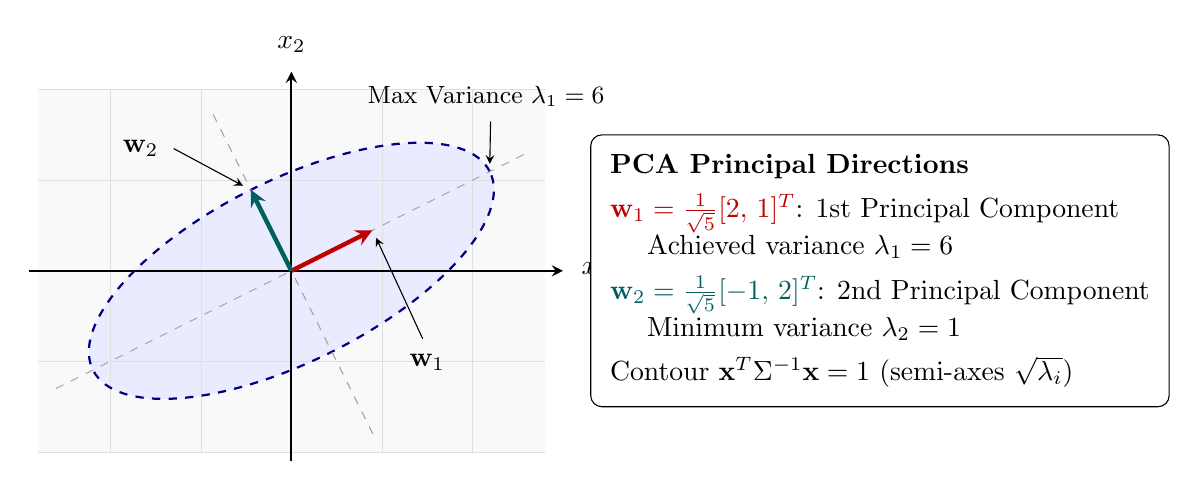
\begin{tikzpicture}[scale=1.15]
        % Layer 1: Background and Covariance Ellipse Fill
        \fill[gray!5] (-2.8,-2.0) rectangle (2.8,2.0);
        \fill[blue!8, rotate=26.565] (0,0) ellipse (2.45 and 1.0);

        % Layer 2: Grid and Axes
        \draw[step=1cm, gray!25, very thin] (-2.8,-2.0) grid (2.8,2.0);
        \draw[->, >=stealth, thick, black] (-2.9,0) -- (3.0,0) node[right=3pt, black] {$x_1$};
        \draw[->, >=stealth, thick, black] (0,-2.1) -- (0,2.2) node[above=3pt, black] {$x_2$};

        % Layer 3: Contour Border, Principal Axes, Vectors, and Callouts
        \draw[blue!50!black, thick, dashed, rotate=26.565] (0,0) ellipse (2.45 and 1.0);
        \draw[dashed, gray!70] (-2.6,-1.3) -- (2.6,1.3);
        \draw[dashed, gray!70] (0.9,-1.8) -- (-0.9,1.8);

        \draw[->, >=stealth, ultra thick, red!75!black] (0,0) -- (0.894, 0.447);
        \draw[->, >=stealth, ultra thick, teal!75!black] (0,0) -- (-0.447, 0.894);

        \draw[->, >=stealth, thin, shorten >=2pt] (1.45, -0.75) -- (0.91, 0.42);
        \draw[->, >=stealth, thin, shorten >=2pt] (-1.3, 1.35) -- (-0.48, 0.91);
        \draw[->, >=stealth, thin, shorten >=2pt] (2.2, 1.65) -- (2.19, 1.12);

        % Layer 4: Labels and Single-Node Legend
        \node[below=2pt, black] at (1.5, -0.75) {$\mathbf{w}_1$};
        \node[left=2pt, black] at (-1.3, 1.35) {$\mathbf{w}_2$};
        \node[above=2pt, black] at (2.15, 1.65) {\small Max Variance $\lambda_1 = 6$};

        \node[draw, rounded corners, fill=white, align=left, inner sep=7pt, anchor=west, text=black] at (3.3, 0.0) {
            \textbf{PCA Principal Directions}\\[4pt]
            \textcolor{red!75!black}{$\mathbf{w}_1 = \frac{1}{\sqrt{5}}[2,\,1]^T$}: 1st Principal Component\\
            \hspace{1em} Achieved variance $\lambda_1 = 6$\\[4pt]
            \textcolor{teal!75!black}{$\mathbf{w}_2 = \frac{1}{\sqrt{5}}[-1,\,2]^T$}: 2nd Principal Component\\
            \hspace{1em} Minimum variance $\lambda_2 = 1$\\[4pt]
            Contour $\mathbf{x}^T\Sigma^{-1}\mathbf{x} = 1$ (semi-axes $\sqrt{\lambda_i}$)
        };
    \end{tikzpicture}
    \end{center}
\end{enumerate}
\textbf{Final Answer:} (a) $\nabla_{\mathbf{w}}\mathcal{L} = \mathbf{0} \implies \Sigma\mathbf{w} = \lambda\mathbf{w}$ and $\mathbf{w}^T\Sigma\mathbf{w} = \lambda$; (b) eigenvalues $6, 1$, maximum variance $6$, $\mathbf{w}_1 = \frac{1}{\sqrt{5}}\begin{bmatrix} 2 \\ 1 \end{bmatrix}$.

\vspace{0.4em}
\textbf{Problem 26:}
In a two-asset portfolio, the weekly return covariance matrix (measured in units of $10^{-4}$) is
\[
\Sigma = \begin{bmatrix} 10 & -3 \\ -3 & 2 \end{bmatrix}.
\]
\begin{enumerate}[label=(\alph*)]
    \item Find the eigenvalues of $\Sigma$, which represent the variances of the two uncorrelated market risk factors.
    \item Find unit eigenvectors $\mathbf{w}_1$ and $\mathbf{w}_2$ for these risk factors and verify algebraically that $\mathbf{w}_1^T \mathbf{w}_2 = 0$.
    \item State the risk factor volatilities (standard deviations) in units of $10^{-2}$.
\end{enumerate}

\textbf{Solution:}
\begin{enumerate}[label=(\alph*)]
    \item Compute $\det(\Sigma - \lambda I) = 0$:
    \[
    \det \begin{bmatrix} 10 - \lambda & -3 \\ -3 & 2 - \lambda \end{bmatrix} = (10 - \lambda)(2 - \lambda) - 9 = \lambda^2 - 12\lambda + 11 = (\lambda - 11)(\lambda - 1) = 0.
    \]
    The eigenvalues are $\lambda_1 = 11$ and $\lambda_2 = 1$ (representing variances $11 \times 10^{-4}$ and $1 \times 10^{-4}$).

    \item \textbf{For $\lambda_1 = 11$:}
    \[
    \Sigma - 11I = \begin{bmatrix} -1 & -3 \\ -3 & -9 \end{bmatrix} \sim \begin{bmatrix} 1 & 3 \\ 0 & 0 \end{bmatrix} \implies x_1 = -3x_2.
    \]
    Setting $x_2 = 1$ gives $\mathbf{v}_1 = \begin{bmatrix} -3 \\ 1 \end{bmatrix}$ with norm $\sqrt{(-3)^2 + 1^2} = \sqrt{10}$, so $\mathbf{w}_1 = \frac{1}{\sqrt{10}}\begin{bmatrix} -3 \\ 1 \end{bmatrix}$.

    \textbf{For $\lambda_2 = 1$:}
    \[
    \Sigma - I = \begin{bmatrix} 9 & -3 \\ -3 & 1 \end{bmatrix} \sim \begin{bmatrix} 1 & -1/3 \\ 0 & 0 \end{bmatrix} \implies x_1 = \frac{1}{3}x_2.
    \]
    Setting $x_2 = 3$ gives $\mathbf{v}_2 = \begin{bmatrix} 1 \\ 3 \end{bmatrix}$ with norm $\sqrt{10}$, so $\mathbf{w}_2 = \frac{1}{\sqrt{10}}\begin{bmatrix} 1 \\ 3 \end{bmatrix}$.

    Orthogonality check:
    \[
    \mathbf{w}_1^T \mathbf{w}_2 = \frac{1}{10}\bigl[(-3)(1) + (1)(3)\bigr] = \frac{-3 + 3}{10} = 0.
    \]

    \item Taking the square roots of the variances $\lambda_1 \times 10^{-4} = 11 \times 10^{-4}$ and $\lambda_2 \times 10^{-4} = 1 \times 10^{-4}$ yields factor volatilities $\sigma_1 = \sqrt{11} \times 10^{-2}$ and $\sigma_2 = 1 \times 10^{-2}$.
\end{enumerate}
\textbf{Final Answer:} (a) $\lambda_1 = 11$, $\lambda_2 = 1$ ($\times 10^{-4}$); (b) $\mathbf{w}_1 = \frac{1}{\sqrt{10}}\begin{bmatrix} -3 \\ 1 \end{bmatrix}$, $\mathbf{w}_2 = \frac{1}{\sqrt{10}}\begin{bmatrix} 1 \\ 3 \end{bmatrix}$, with $\mathbf{w}_1^T\mathbf{w}_2 = 0$; (c) $\sigma_1 = \sqrt{11} \times 10^{-2}$, $\sigma_2 = 10^{-2}$.

\vspace{0.4em}
\textbf{Problem 27:}
A small three-page web network is modeled by the column-stochastic transition matrix
\[
P = \begin{bmatrix} 0 & 1 & 1/2 \\ 1/2 & 0 & 0 \\ 1/2 & 0 & 1/2 \end{bmatrix},
\]
where entry $P_{ij}$ gives the probability of transitioning from page $j$ to page $i$.
\begin{enumerate}[label=(\alph*)]
    \item Verify that $\lambda = 1$ is an eigenvalue of $P$ and find a basis for the steady-state eigenspace $E_1$.
    \item Find the unique steady-state probability vector $\boldsymbol{\pi} \in E_1$ whose components sum to $1$, and rank the three webpages by PageRank importance.
\end{enumerate}

\textbf{Solution:}
\begin{enumerate}[label=(\alph*)]
    \item Construct $P - I$ and row reduce $(P - I)\mathbf{x} = \mathbf{0}$:
    \begin{align*}
    P - I = \begin{bmatrix} -1 & 1 & 1/2 \\ 1/2 & -1 & 0 \\ 1/2 & 0 & -1/2 \end{bmatrix}
    &\xrightarrow{\substack{R_1 \leftarrow -R_1 \\ R_2 \leftarrow 2R_2 \\ R_3 \leftarrow 2R_3}}
    \begin{bmatrix} 1 & -1 & -1/2 \\ 1 & -2 & 0 \\ 1 & 0 & -1 \end{bmatrix} \\
    &\xrightarrow{\substack{R_2 \leftarrow R_2 - R_1 \\ R_3 \leftarrow R_3 - R_1}}
    \begin{bmatrix} 1 & -1 & -1/2 \\ 0 & -1 & 1/2 \\ 0 & 1 & -1/2 \end{bmatrix} \\
    &\xrightarrow{\substack{R_3 \leftarrow R_3 + R_2 \\ R_2 \leftarrow -R_2 \\ R_1 \leftarrow R_1 + R_2}}
    \begin{bmatrix} 1 & 0 & -1 \\ 0 & 1 & -1/2 \\ 0 & 0 & 0 \end{bmatrix}.
    \end{align*}
    Because $x_3$ is a free variable, $(P - I)\mathbf{x} = \mathbf{0}$ has nontrivial solutions, confirming $\lambda = 1$ is an eigenvalue. The equations $x_1 = x_3$ and $x_2 = \frac{1}{2}x_3$ with $x_3 = 2$ (clearing fractions) produce the basis $\left\{ \begin{bmatrix} 2 \\ 1 \\ 2 \end{bmatrix} \right\}$ for $E_1$.

    \item Every vector in $E_1$ has the form $\mathbf{x} = t\begin{bmatrix} 2 \\ 1 \\ 2 \end{bmatrix}$. Imposing the probability normalization $\pi_1 + \pi_2 + \pi_3 = 1$ gives $t(2 + 1 + 2) = 5t = 1 \implies t = \frac{1}{5}$. Thus the unique steady-state PageRank vector is
    \[
    \boldsymbol{\pi} = \begin{bmatrix} 2/5 \\ 1/5 \\ 2/5 \end{bmatrix} = \begin{bmatrix} 0.4 \\ 0.2 \\ 0.4 \end{bmatrix}.
    \]
    Pages $1$ and $3$ tie for highest importance ($\pi_1 = \pi_3 = 0.4$), while Page $2$ ranks lowest ($\pi_2 = 0.2$).
\end{enumerate}
\textbf{Final Answer:} (a) $\lambda = 1$ verified with $E_1$ basis $\left\{ \begin{bmatrix} 2 \\ 1 \\ 2 \end{bmatrix} \right\}$; (b) $\boldsymbol{\pi} = \begin{bmatrix} 2/5 \\ 1/5 \\ 2/5 \end{bmatrix}$ (Pages $1$ and $3$ tied for first, Page $2$ third).

\vspace{0.4em}
\textbf{Problem 28:}
Consider the coupled linear differential system $\mathbf{x}'(t) = A\mathbf{x}(t)$ with initial state $\mathbf{x}(0)$, where
\[
A = \begin{bmatrix} -4 & 2 \\ 1 & -3 \end{bmatrix}, \quad \mathbf{x}(0) = \begin{bmatrix} 3 \\ 0 \end{bmatrix}.
\]
\begin{enumerate}[label=(\alph*)]
    \item Find the eigenvalues and corresponding eigenvectors of $A$.
    \item Using the general solution $\mathbf{x}(t) = c_1 e^{\lambda_1 t}\mathbf{v}_1 + c_2 e^{\lambda_2 t}\mathbf{v}_2$, determine the exact trajectory $\mathbf{x}(t)$ satisfying the given initial condition $\mathbf{x}(0)$.
    \item Based on the eigenvalues, classify the long-term behavior of $\mathbf{x}(t)$ as $t \to \infty$ (decays to zero, oscillates, or explodes to infinity).
\end{enumerate}

\textbf{Solution:}
\begin{enumerate}[label=(\alph*)]
    \item Solve $\det(A - \lambda I) = 0$:
    \[
    \det \begin{bmatrix} -4 - \lambda & 2 \\ 1 & -3 - \lambda \end{bmatrix} = (\lambda + 4)(\lambda + 3) - 2 = \lambda^2 + 7\lambda + 10 = (\lambda + 2)(\lambda + 5) = 0.
    \]
    Thus $\lambda_1 = -2$ and $\lambda_2 = -5$.
    \begin{itemize}
        \item For $\lambda_1 = -2$: $A + 2I = \begin{bmatrix} -2 & 2 \\ 1 & -1 \end{bmatrix} \sim \begin{bmatrix} 1 & -1 \\ 0 & 0 \end{bmatrix} \implies \mathbf{v}_1 = \begin{bmatrix} 1 \\ 1 \end{bmatrix}$.
        \item For $\lambda_2 = -5$: $A + 5I = \begin{bmatrix} 1 & 2 \\ 1 & 2 \end{bmatrix} \sim \begin{bmatrix} 1 & 2 \\ 0 & 0 \end{bmatrix} \implies \mathbf{v}_2 = \begin{bmatrix} -2 \\ 1 \end{bmatrix}$.
    \end{itemize}

    \item Evaluate the general solution at $t = 0$:
    \[
    \mathbf{x}(0) = c_1 \begin{bmatrix} 1 \\ 1 \end{bmatrix} + c_2 \begin{bmatrix} -2 \\ 1 \end{bmatrix} = \begin{bmatrix} 3 \\ 0 \end{bmatrix} \implies \begin{cases} c_1 - 2c_2 = 3 \\ c_1 + c_2 = 0 \end{cases}.
    \]
    Subtracting gives $-3c_2 = 3 \implies c_2 = -1$ and $c_1 = 1$. Therefore,
    \[
    \mathbf{x}(t) = e^{-2t}\begin{bmatrix} 1 \\ 1 \end{bmatrix} - e^{-5t}\begin{bmatrix} -2 \\ 1 \end{bmatrix} = \begin{bmatrix} e^{-2t} + 2e^{-5t} \\ e^{-2t} - e^{-5t} \end{bmatrix}.
    \]

    \item Because both eigenvalues $\lambda_1 = -2 < 0$ and $\lambda_2 = -5 < 0$ are real and strictly negative, both exponential modes $e^{-2t} \to 0$ and $e^{-5t} \to 0$ as $t \to \infty$. Thus $\mathbf{x}(t) \to \mathbf{0}$ monotonically without oscillation (the origin is asymptotically stable).
\end{enumerate}
\textbf{Final Answer:} (a) $\lambda_1 = -2$ ($\mathbf{v}_1 = \begin{bmatrix} 1 \\ 1 \end{bmatrix}$), $\lambda_2 = -5$ ($\mathbf{v}_2 = \begin{bmatrix} -2 \\ 1 \end{bmatrix}$); (b) $\mathbf{x}(t) = \begin{bmatrix} e^{-2t} + 2e^{-5t} \\ e^{-2t} - e^{-5t} \end{bmatrix}$; (c) decays to $\mathbf{0}$ as $t \to \infty$.

\subsection{Advanced Diagnostic Error Analysis (Problems 29--30)}

\textbf{Problem 29:}
You are the grader. Each student solution below contains a single subtle conceptual or algebraic flaw. For each part, (i) identify the flaw in one clear sentence, (ii) provide the corrected mathematical step, and (iii) state the correct final answer.
\begin{enumerate}[label=(\alph*)]
    \item \textbf{Question:} Find all eigenvalues of $A = \begin{bmatrix} 3 & 6 \\ 1 & 4 \end{bmatrix}$.\\
    \textbf{Flawed Solution:} ``Apply the row operation $R_2 \leftarrow 3R_2 - R_1$ to reduce $A$ to $\begin{bmatrix} 3 & 6 \\ 0 & 6 \end{bmatrix}$. Since the reduced matrix is upper triangular, the eigenvalues are the diagonal entries $\lambda = 3$ and $\lambda = 6$.''
    \item \textbf{Question:} Is $\mathbf{v} = \begin{bmatrix} 0 \\ 0 \\ 0 \end{bmatrix}$ an eigenvector of $B = \begin{bmatrix} 2 & -1 & 4 \\ 0 & 5 & 1 \\ 3 & 2 & -1 \end{bmatrix}$?\\
    \textbf{Flawed Solution:} ``Computing $B\mathbf{v} = \begin{bmatrix} 0 \\ 0 \\ 0 \end{bmatrix} = 7\mathbf{v}$, the equation $B\mathbf{v} = \lambda\mathbf{v}$ holds true for $\lambda = 7$ (and every scalar). Therefore, $\mathbf{v}$ is an eigenvector of $B$.''
\end{enumerate}

\textbf{Solution:}
\begin{enumerate}[label=(\alph*)]
    \item \begin{itemize}
        \item \textbf{The Flaw:} Elementary row operations change the eigenvalues of a matrix, so one cannot row-reduce $A$ before finding its eigenvalues.
        \item \textbf{Correct Step:} Solve the characteristic equation $\det(A - \lambda I) = (3 - \lambda)(4 - \lambda) - 6 = \lambda^2 - 7\lambda + 6 = 0$.
        \item \textbf{Correct Answer:} Factoring $(\lambda - 6)(\lambda - 1) = 0$ gives the true eigenvalues $\lambda = 6$ and $\lambda = 1$.
    \end{itemize}
    \item \begin{itemize}
        \item \textbf{The Flaw:} By strict mathematical definition, an eigenvector must be a nonzero vector ($\mathbf{v} \neq \mathbf{0}$).
        \item \textbf{Correct Step:} Recognize immediately that $\mathbf{v} = \mathbf{0}$ fails the nonzero condition in $B\mathbf{v} = \lambda\mathbf{v}$.
        \item \textbf{Correct Answer:} No, the zero vector $\mathbf{0}$ is never an eigenvector of any matrix.
    \end{itemize}
\end{enumerate}
\textbf{Final Answer:} (a) True eigenvalues are $\lambda = 6, 1$; (b) No, $\mathbf{0}$ is never an eigenvector.

\vspace{0.4em}
\textbf{Problem 30:}
You are the grader. Each student solution below contains a single subtle conceptual or algebraic flaw. For each part, (i) identify the flaw in one clear sentence, (ii) provide the corrected mathematical step, and (iii) state the correct final answer.
\begin{enumerate}[label=(\alph*)]
    \item \textbf{Question:} Find a basis for the eigenspace of $A = \begin{bmatrix} 7 & -4 \\ 0 & 7 \end{bmatrix}$ corresponding to $\lambda = 7$.\\
    \textbf{Flawed Solution:} ``We compute $A - 7I = \begin{bmatrix} 0 & -4 \\ 0 & 0 \end{bmatrix}$, which gives $-4x_2 = 0$, so $x_2 = 0$. Therefore, the only solution is $\mathbf{x} = \mathbf{0}$, and $A$ has no eigenvectors for $\lambda = 7$.''
    \item \textbf{Question:} Suppose $C\mathbf{x} = \mathbf{0}$ for some nonzero vector $\mathbf{x} \in \mathbb{R}^3$. Does $C$ have an eigenvalue corresponding to $\mathbf{x}$?\\
    \textbf{Flawed Solution:} ``Because $C$ maps $\mathbf{x}$ to the zero vector, there is no nonzero scalar $\lambda$ stretching or compressing $\mathbf{x}$. Hence, $C$ has no eigenvalue for $\mathbf{x}$.''
    \item \textbf{Question:} Find a basis for the eigenspace of $D = \begin{bmatrix} -1 & 4 \\ 1 & -1 \end{bmatrix}$ corresponding to $\lambda = -3$.\\
    \textbf{Flawed Solution:} ``Constructing $D - (-3)I = \begin{bmatrix} 2 & 4 \\ 1 & 2 \end{bmatrix} \sim \begin{bmatrix} 1 & 2 \\ 0 & 0 \end{bmatrix}$ yields $x_1 + 2x_2 = 0$, so $x_1 = 2x_2$. Taking $x_2$ free gives the basis $\left\{ \begin{bmatrix} 2 \\ 1 \end{bmatrix} \right\}$.''
\end{enumerate}

\textbf{Solution:}
\begin{enumerate}[label=(\alph*)]
    \item \begin{itemize}
        \item \textbf{The Flaw:} The student overlooked that column $1$ of $A - 7I$ contains no pivot, making $x_1$ a free variable.
        \item \textbf{Correct Step:} With $x_2 = 0$ and $x_1$ free, write the solution in parametric vector form $\mathbf{x} = x_1 \begin{bmatrix} 1 \\ 0 \end{bmatrix}$.
        \item \textbf{Correct Answer:} The basis for the eigenspace $E_7$ is $\left\{ \begin{bmatrix} 1 \\ 0 \end{bmatrix} \right\}$.
    \end{itemize}
    \item \begin{itemize}
        \item \textbf{The Flaw:} The student mistakenly assumes that a scalar factor of zero cannot be a valid eigenvalue.
        \item \textbf{Correct Step:} Rewrite $C\mathbf{x} = \mathbf{0}$ explicitly as $C\mathbf{x} = 0 \cdot \mathbf{x}$ with $\mathbf{x} \neq \mathbf{0}$.
        \item \textbf{Correct Answer:} Yes, $C$ has an eigenvalue corresponding to $\mathbf{x}$, namely $\lambda = 0$.
    \end{itemize}
    \item \begin{itemize}
        \item \textbf{The Flaw:} The student made a sign error when isolating $x_1$ from $x_1 + 2x_2 = 0$, writing $x_1 = 2x_2$ instead of $x_1 = -2x_2$.
        \item \textbf{Correct Step:} Solve $x_1 + 2x_2 = 0 \implies x_1 = -2x_2$, yielding $\mathbf{x} = x_2 \begin{bmatrix} -2 \\ 1 \end{bmatrix}$.
        \item \textbf{Correct Answer:} The correct basis for $E_{-3}$ is $\left\{ \begin{bmatrix} -2 \\ 1 \end{bmatrix} \right\}$.
    \end{itemize}
\end{enumerate}
\textbf{Final Answer:} (a) $\left\{ \begin{bmatrix} 1 \\ 0 \end{bmatrix} \right\}$; (b) Yes, $\lambda = 0$; (c) $\left\{ \begin{bmatrix} -2 \\ 1 \end{bmatrix} \right\}$.

\newpage

\section{Master Concept Checklist and Quick Reference}

For rapid review and targeted exam preparation, the full concept-to-problem mapping is reproduced below.

\renewcommand{\arraystretch}{1.5}
\begin{tabularx}{\textwidth}{>{\bfseries\raggedright\arraybackslash}p{3.6cm} >{$\displaystyle}l<{$} >{\raggedright\arraybackslash}X >{\raggedright\arraybackslash}p{2.5cm}}
\toprule
\textbf{Concept / Problem Type} & \text{\textbf{Core Formula / Criterion}} & \textbf{Key Skills and Edge Cases Tested} & \textbf{Problem(s)} \\
\midrule
Core Definition and Geometry & A\mathbf{x} = \lambda\mathbf{x},\ \mathbf{x} \neq \mathbf{0} & Scaling along invariant spans; rejecting the zero vector $\mathbf{0}$; reversing direction ($\lambda < 0$). & 1, 2, 13, 29(b) \\
Verifying an Eigenvector & A\mathbf{v} = \lambda\mathbf{v} & Direct multiplication in $\mathbb{R}^2$ and $\mathbb{R}^3$; checking scalar consistency across components; $\lambda = 0$ case. & 1, 2, 3 \\
Verifying an Eigenvalue & (A - \lambda I)\mathbf{x} = \mathbf{0} & Matrix shifting; row reducing to check for free variables; avoiding sign errors when subtracting negative diagonal entries. & 4, 5 \\
Eigenspace Basis Extraction & \operatorname{Nul}(A - \lambda I) & Converting RREF to parametric vector form; fraction clearing to obtain clean integer basis vectors. & 6, 7, 8, 9, 10, 12, 30(a), 30(c) \\
Multi-Dimensional Eigenspaces and Leading Free Variables & \dim E_\lambda \ge 1 & Identifying $2$D plane eigenspaces; recognizing when $x_1$ has no pivot and is a free variable. & 8, 9, 17, 30(a) \\
Characteristic Equation and Full Spectrum & \det(A - \lambda I) = 0 & Computing characteristic polynomials for $2\times 2$ and $3\times 3$ matrices; finding all eigenvalues and bases. & 12, 13, 14, 15, 16, 24, 25, 26, 28, 29(a) \\
Triangular Matrix Shortcut & \det(A - \lambda I) = \prod (a_{ii} - \lambda) & Reading eigenvalues directly from main diagonals of upper/lower triangular matrices without row reducing $A$. & 10, 17, 22 \\
Zero Eigenvalue and Invertibility & \lambda = 0 \iff \det(A) = 0 & Connecting $\lambda = 0$ to singular matrices, dependent columns, and nontrivial null spaces. & 3, 10, 11, 20, 30(b) \\
Complex Eigenvalues and Rotations & \lambda = \alpha \pm \beta i \in \mathbb{C} & Solving $\det(A - \lambda I) = 0$ over $\mathbb{C}$; interpreting absence of real eigenvectors for rotation matrices $R_\theta$. & 13, 14, 15 \\
Algebraic vs.\ Geometric Multiplicity & \operatorname{GM}(\lambda) \le \operatorname{AM}(\lambda) & Comparing root multiplicity to eigenspace dimension; classifying defective matrices; parameter tuning. & 10, 16, 17, 18 \\
Theoretical Proofs and Matrix Algebra & p(A)\mathbf{x} = p(\lambda)\mathbf{x} & Independence of distinct-eigenvalue vectors; $A^{-1}$, $A+cI$, $A^k$, $A^T$, idempotent, nilpotent, and eigenbasis powers. & 19, 20, 21, 22, 23, 24 \\
Real-World Modeling (ML, Quant, Markov, ODEs) & \Sigma\mathbf{w} = \lambda\mathbf{w},\ P\boldsymbol{\pi} = \boldsymbol{\pi} & PCA variance maximization via Lagrange multipliers; portfolio risk factors; PageRank steady state; ODE stability. & 25, 26, 27, 28 \\
Diagnostic Testing (``Find the Flaw'') & \text{Row ops alter } \lambda & Catching row reduction of $A$, zero-vector traps, missed free variables, $\lambda = 0$ myths, and sign errors. & 4, 9, 29, 30 \\
\bottomrule
\end{tabularx}

\end{document}